\documentclass[times,doublespace]{fldauth}

\usepackage{hyperref}
\usepackage{lineno}
\usepackage{amsmath}
\usepackage{amssymb}
\usepackage{graphicx}

\newcommand{\vb}{\mathbf}
\newcommand{\vg}{\boldsymbol}
\newcommand{\diff}[2]{\frac{d #1}{d #2}}
\newcommand{\pdiff}[2]{\frac{\partial #1}{\partial #2}}
\newcommand{\avg}[1]{\overline{#1}}
\newcommand{\dblavg}[1]{\overline{\overline{#1}}}
\newcommand{\mat}[1]{\mathbf{\mathsf{#1}}}
\newcommand{\arccot}{\mathrm{arccot}}

\newcommand{\rbd}[1]{\raisebox{-1.5ex}[1.5ex]{#1}}
\newcommand{\rbu}[1]{\raisebox{0.5ex}[-0.5ex]{#1}}
\newcommand{\rb}[1]{\raisebox{2ex}[-2ex]{#1}}

\newcommand\T{\rule{0pt}{2.6ex}}
\newcommand\B{\rule[-1.2ex]{0pt}{0pt}}


\begin{document}
\setcounter{section}{-1}

\title{Dynamical Core Model Intercomparison Project (DCMIP2016) \\
 Test Case Document}
\author{Paul Aaron Ullrich \\Antonin Verlet-Banide\\ Christiane Jablonowski \\ Kevin Reed \\ Colin Zarzycki \\ Peter Hjort Lauritzen \\ Ramachandran D. Nair \\ James Kent \\ \vspace{3cm} DCMIP Summer School: June 2016}

\maketitle

\begin{center}
Version 0.2 \\
\today
\end{center}

\vspace{2cm}

\begin{center}
Email questions to \textbf{dcmip@ucar.edu}
\end{center}

\clearpage

\section*{Overview of the Test Case Suite}

The set of test cases collected in this document has been developed for the 2016 Dynamical Core Model Intercomparison Project (DCMIP2016) in an effort to understand the broad treatment of the equations of motion within a variety of atmospheric General Circulation Models (GCMs). In contrast with the test cases described in the DCMIP2012 and DCMIP2008 test case documents, the suite of test cases that are described here focus on issues related to physics-dynamics coupling, non-hydrostatic scales and modeling systems that support variable resolution.  To better isolate these features, the majority of tests described in this document do not include topographic forcing and emphasize features that have a relatively small spatial footprint relative to the global simulation domain.  The tests proposed here have been drawn from the recent literature on global model intercomparison testing.  To support the integration of these tests into existing models, a collection of initialization routines have been provided that can be used for very quickly setting up the initial conditions.  Augmented Kessler physics routines have also been provided to support simple moisture feedbacks, a boundary layer parameterization and surface friction.  If models provide both a shallow-atmosphere and deep-atmosphere configuration, we recommend the shallow-atmosphere setup to avoid imbalances in the initial conditions. It is further expected that most models will be run under a non-hydrostatic configuration, which will permit a correct solution to the mesoscale storm test.  If models can be configured both as a hydrostatic and non-hydrostatic dynamical core, additional hydrostatic simulations might be conducted to evaluate the direct impact of the hydrostatic approximation.  Table \ref{tab:TestCases} provides an overview of all test cases described in this document.

\begin{table}[h]

\caption{A list of test cases described in this document.} \label{tab:TestCases}
%\ \\
\begin{tabular*}{\textwidth}{@{\extracolsep{\fill}}ll}
\hline Test Case \T \B& Description \\
\hline \multicolumn{2}{l}{Tier 1 Test Cases (Required)} \T \B \\
\hline 
1-1 \T & Moist baroclinic wave with terminator chemistry \\
1-2 \T & Idealized Tropical cyclone \\
1-3 \T & Mesoscale storm \\
%1-4 \T & Steady-state Terminator chemistry (pure advection) \\
\hline \multicolumn{2}{l}{Tier 2 Test Cases (Optional)} \T \B \\  \hline 
2-1 \T \B & Moist Held-Suarez test  \\ \hline
\hline 
\end{tabular*}

\end{table}

\section{Practical Considerations}

\subsection{List of Symbols}
Throughout this test case document we will use $\lambda \in [0, 2 \pi)$ to denote longitude, $\varphi \in [-\pi/2, \pi/2]$ to represent latitude, $z$ to represent the height with respect to the mean sea level (assumed to be zero), and $p$ to symbolize the pressure. Table \ref{tab:symbols} lists the symbols used for the initialization of the model.

\begin{table}[h]
\caption{List of symbols for the model initialization} \label{tab:symbols}
\begin{center}
\begin{tabular}{cl}
\hline Symbol & Description \\ \hline 
$\lambda$ & Longitude (in radians) \\
$\varphi$ & Latitude (in radians) \\
$z$ & Height with respect to mean sea level (set to zero) \\
$p_s$ & Surface pressure ($p_s$ of moist air if $q>0$) \\
$\Phi_s$ & Surface geopotential \\
$z_s$ & Surface elevation with respect to mean sea level (set to zero) \\
$u$ & Zonal wind \\
$v$ & Meridional wind \\
$w$ & Vertical velocity \\
$\omega$ & Vertical pressure velocity  \\
$\delta$ & Divergence\\
$\zeta$ & Relative vorticity\\
$p$ & Pressure (pressure of moist air if $q>0$) \\
$\rho$ & Density (density of moist air if $q>0$)\\
$T$ &Temperature \\
$T_v$ & Virtual temperature \\
$\Theta$ & Potential temperature \\
$\Theta_v$ & Virtual potential temperature \\
$q$ & Specific humidity \\
$P_{ls}$ & Large-scale precipitation rate \\
$q_c$ & Cloud water mixing ratio \\
$q_r$ & Rain water mixing ratio \\
$q_{Cl}$ & Singlet chlorine mixing ratio \\
$q_{Cl2}$ & Chlorine gas mixing ratio \\
\hline 
\end{tabular}
\end{center}
\end{table}

\subsection{List of Physical Constants}
A list of physical constants which are used throughout this document is given in Table \ref{tab:PhysicalConstants}.  Constants which are specific to each test case are similarly tabulated at the beginning of each section.

\begin{table}[h]
\caption{A list of physical constants used in this document.} \label{tab:PhysicalConstants}
%\ \\
\begin{tabular*}{\textwidth}{@{\extracolsep{\fill}}lll}
\hline Constant & Description & Value \\
\hline $a_{\tiny \mbox{ref}}$ & Radius of the Earth & $6.37122 \times 10^{6}\ \mbox{m}$ \\
$\Omega_{\tiny \mbox{ref}}$ & Rotational speed of the Earth & $7.292\ \times 10^{-5}\ \mbox{s}^{-1}$ \\
$X$ & Reduced-size Earth reduction factor & variable (default $= 1$) \\
$a$ & Scaled radius of the Earth & $a_{\tiny \mbox{ref}} / X$ \\
$\Omega$ & Scaled rotational speed of the Earth & $\Omega_{\tiny \mbox{ref}} \cdot X$ \\
$g$ & Gravity & $9.80616\ \mbox{m}\ \mbox{s}^{-2}$ \\
$p_0$ & Reference pressure & $1000\ \mbox{hPa}$ \\
$c_p$ & Specific heat capacity of dry air at constant pressure & $1004.5\ \mbox{J}\ \mbox{kg}^{-1}\ \mbox{K}^{-1}$ \\
$c_v$ & Specific heat capacity of dry air at constant volume & $717.5\ \mbox{J}\ \mbox{kg}^{-1}\ \mbox{K}^{-1}$ \\
$R_d$ & Gas constant for dry air & $287.0\ \mbox{J}\ \mbox{kg}^{-1}\ \mbox{K}^{-1}$ \\
$R_\nu$ & Gas constant for water vapor & $461.5$ J kg$^{-1}$ K$^{-1}$ \\
$\kappa$ & Ratio of $R_d$ to $c_p$ & $R_d/c_p = 2/7$ \\
$\varepsilon$ & Ratio of $R_d$ to $R_\nu$ & $R_d/R_\nu \approx 0.622$ \\
$M_v$ & Constant for virtual temperature conversion & $0.608$ \\
$\rho_{water}$ & Density of water & 1000 kg m$^{-3}$ \\
\hline 
\end{tabular*}

\end{table}

\subsection{Great Circle Distance}

The great circle distance is used throughout the document and is given by
\begin{equation}
R_c(\lambda_1, \varphi_1; \lambda_2, \varphi_2) = a \arccos \left( \sin \varphi_1 \sin \varphi_2 + \cos \varphi_1 \cos \varphi_2 \cos (\lambda_1 - \lambda_2) \right).
\end{equation}

\subsection{Choice of Prognostic Variables and Equation of State}

It is assumed throughout this document that the moist ideal gas law is satisfied,
\begin{equation} \label{eq:idealgaslaw}
p = \rho R_d T_v, 
\end{equation} where the virtual temperature is defined in terms of the temperature as
\begin{equation} \label{eq:virtualtemperature}
T_v = T (1 + M_v q).
\end{equation}  The virtual potential temperature is similarly related to the potential temperature via the relationship
\begin{equation}
\theta_v = \theta (1 + M_v q).
\end{equation}

\subsection{Small-Planet Experiments}
The test case suite makes use of small-planet experiments that have the potential to expose the differences between hydrostatic and non-hydrostatic modeling approaches at reasonable computational cost. In particular, the small-planet setups allow the evaluation of the model behavior with physical grid spacings down to a few hundred meters. In some instances, we suggest small planets with circumferences of about 40 km and a vertical extent of 30 km which raises questions concerning the validity of the shallow-atmosphere approximation. However, since the experiments are not compared to observations, we still ask for the use of the shallow-atmosphere approach to allow for intercomparisons among the DCMIP models and to avoid imbalances of the initial conditions.

When a non-unity reduction factor $X$ is applied in order to shrink the size of the Earth and thereby the physical grid spacing of the computational grid, a variety of model adjustments become necessary.
Most prominently these include the scaling of the radius, the rotational speed, the model time step and explicit viscosity parameters (if applied). The adjustment steps for small-planet simulations are:
\begin{itemize}
\item Divide the radius of the Earth $a_{\tiny \mbox{ref}}$ by $X$ to obtain the rescaled radius $a  = \frac{a_{\tiny \mbox{ref}}}{X}$.
\item Divide the length of the dynamics time step $\Delta t$ by $X$, especially if a CFL condition needs to be obeyed.
\item In case of rotating planets: multiply the Earth's angular velocity $\Omega_{\tiny \mbox{ref}}$ by the factor $X$ to obtain the rescaled angular speed $\Omega = \Omega_{\tiny \mbox{ref}}X$. This guarantees that the characteristics of Rossby waves are comparable in unscaled and scaled model experiments since the Rossby number stays constant.
\item In case of explicit diffusion of type $K_{2k}\nabla^{2k}$ with a prescribed diffusion coefficient $K_{2k}$ (and $k=1,2\ldots$) divide $K_{2k}$ by the factor $X^{2k-1}$. This accounts for a reduction of the e-folding time $\tau$  and the horizontal grid spacing $\Delta x$ according to the relationship $\frac{(\Delta x)^{2k}/X^{2k}}{\tau/X}$. The $K_{2k}$ diffusion coefficient is typically based on such a relationship. Note that some models might provide an automatic scaling of the diffusion coefficients according to the actual dynamics time step and grid spacing. If a model applies Rayleigh friction as a sponge near the model top, the friction coefficient needs to be multiplied by X. Again, this corresponds to a reduction of the e-folding frictional time scale $\frac{1}{\tau/X} = \frac{X}{\tau}$ in small-planet experiments.
\item If physical forcing mechanisms are present on the right hand side of the equations of motion the strengths of the physical forcing must be increased (multiplied) by the factor X. This will not be applicable to the test cases presented here unless Rayleigh friction is considered as such a forcing as outlined above.
\end{itemize}

\subsection{Notes on the Requested Model Output}
\label{sec:notes_output}
\subsubsection{NetCDF}
A fundamental requirement for the exchange of scientific data is the ability to  precisely describe the physical quantities being represented. Therefore, special attention needs to be paid to the representation of the model data in the output files. We require data in the `Network Common Data Form' (netCDF) \cite{netcdf} that adhere to the netCDF Climate and Forecast (CF) metadata convention (if possible to version 1.6 from Dec. 2011 \cite{netcdf-cf}). All netCDF files should have the file name extension `.nc'.
We specify details of the netCDF requirements in Appendix~\ref{sec:netcdf} and will also provide help via NCO operators before the DCMIP event to make the data CF-compliant if necessary. Please communicate your output constraints or concerns (if any) to the DCMIP organizers as soon as possible. We will also ask for example data sets before the DCMIP event.

\subsubsection{Computational grid}
Most DCMIP models utilize non-orthogonal computational grids like cubed-sphere grids, icosahedral grids, hexagonal grid, Voronoi grids or Yin-Yang grids. Among the mix of DCMIP GCMs are even models that provide provisions for variable-resolution grids. We encourage the use of the variable-resolution configurations as an additional test option whenever possible.
This raises questions concerning the desired representation of the data in the netCDF output files. 

If models on non-traditional (non latitude-longitude) grids are used, we ask for two output files that represent the identical model run. The first output file should be written on the native computational grid without any interpolations. In addition, most models will likely provide built-in provisions for interpolated output to a regular (equidistant in degrees) latitude-longitude grid. We therefore also ask for a second output file that represents the data on model levels on the interpolated latitude-longitude grid. We ask for co-located  (Arakawa-A type) data on the interpolated grid regardless of the GCM's staggering options. The grid spacing of the interpolated grid should be comparable to the actual resolution of the model run, which might be for example $1^\circ \times 1^\circ$. Using this example, the interpolated grid will have $180 \times 360$ horizontal grid points if the equator and pole points are not part of the interpolated grid. If the equator and pole points are included it yields $181 \times 360$ horizontal grid points. If models can freely choose their interpolation points, we suggest the $180 \times 360$ configuration for the given example. If models need to include the equator and pole points, we ask for the $181 \times 360$ horizontal grid. 

Models on regular latitude-longitude or Gaussian grids should only provide a single output file using their native horizontal resolution and model levels. If reduced Gaussian grids are utilized a second file on the full Gaussian grid is requested. 
If models are run with variable-resolution grids, we leave the choice of the best suitable interpolation grid to the modeling group. We ask to write all output variables for each experiment to the same file.

\subsection{Short Note on Data Analysis and Visualization}
We will provide NCAR Command Language (NCL) scripts to help visualize the model results and provide analysis functions. In addition, the DCMIP participants will have access to interactive Graphical User Interfaces (GUIs) to support the visualization and model intercomparison. Among the GUIs are the netCDF viewers Ncview and Panoply which are public domain tools and locally installed on the NCAR mirage server. In addition, we expect to provide some basic online visualization capabilities via NOAA's Live Access Server (LAS) software. A key to the successful visualization is the adherence of the output data sets to the netCDF-CF standard (see Appendix \ref{sec:netcdf}).

\subsection{Short Note on the Fortran Templates}
\label{sec:template}
We have provided a set of stand-alone Fortran routines that compute the initial conditions for all test cases. They are named

\begin{itemize}
\item \texttt{baroclinic\_wave\_test.f90}
\item \texttt{tropical\_cyclone\_test.f90}
\item \texttt{mesoscale\_storm\_test.f90}
\end{itemize}

We have also provided a set of stand-alone Fortran routines that compute tendencies associated with the physical parameterizations.  They are named

\begin{itemize}
\item \texttt{terminator.f90}
\item \texttt{kessler.f90}
\end{itemize}

%%%%%%%%%%%%%%%%%%%%%%%%%%%%%%%%%%%%%%%%%%%%%%%%%%%%%%%%%%%%%%%%%%%%%%%%%%%%%%%%%%%%%%%%%%%%%%%%%%%%%%%%%%%%%%%%%%%%%%%%%%%%%%%%%%

\clearpage
\section{Moist Baroclinic Wave} \label{sec:baroclinic_wave}
 
This baroclinic instability test of \cite{ullrich2014proposed} considers a reference state in geostrophic and hydrostatic balance that satisfies the conditions for baroclinic instability.  Although a perfect model should be able to maintain this state indefinitely, small truncation errors associated with numerical inaccuracies and grid structure will trigger the development of the wave modes associated with baroclinic development.  To control the development of the baroclinic wave, a small perturbation (but one which is large compared with machine truncation) is added to the flow so as to trigger the development of a wave over a period of approximately 10 days.  A moist variant of the dry dynamical test of \cite{ullrich2014proposed} is considered here so as to understand the impact of moisture feedbacks on the development of the wave.

This test case is similar in character to the test of \cite{jablonowski2006baroclinic}, but has a number of key differences:  (1) this test is an analytical solution of the equations of motion in height ($z$) coordinates, (2) the bottom topography is zero throughout the domain, (3) the new test case does not have a distinct stratosphere (the presence of a stratosphere is largely irrelevant for understanding baroclinic development), and (4) the velocity field goes to zero at the model surface.
 
\begin{table}[h]

\caption{List of constants used for the Moist Baroclinic Wave test case}
\label{test4:tab}
\begin{tabular*}{\textwidth}{@{\extracolsep{\fill}}lll}
\hline Constant & Value & Description \\
\hline 
$z_{\tiny \mbox{top}}$ & $44000\ \mbox{m}$ & Recommended height position of the model top \\
$p_{\tiny \mbox{top}}$ & $\approx 2.26$ hPa & Recommended pressure at the model top\\
$X$ & $1$ & Reduced-size planet scaling factor, see below\\
$a$ & $a_{\tiny \mbox{ref}}/X$ & Scaled radius of the Earth \\
$\Omega$ & $\Omega_{\tiny \mbox{ref}}X$ & Scaled angular speed of the Earth \\
$p_s$ & $1000\ \mbox{hPa}$ & Surface pressure (constant) \\
$p_0$ & $1000\ \mbox{hPa}$ & Reference pressure (constant) \\
$u_0$ & $35\ \mbox{m\ s}^{-1}$ & Maximum amplitude of the zonal wind \\
$b$ & $2$ & Half-width parameter \\
$K$ & $3$ & Power used for temperature field \\
$T_E$ & $310\ \mbox{K}$ & Horizontal-mean temperature at the surface \\
$T_P$ & $240 \ \mbox{K}$ & Temperature at the polar surface\\
$u_p$ & $1\ \mbox{m\ s}^{-1}$ & Maximum amplitude of the zonal wind perturbation \\
$z_p$ & $15000\ \mbox{m}$ & Maximum height of the zonal wind perturbation \\
$\lambda_p$ & $\pi / 9$ & Longitude of the zonal wind perturbation centerpoint (20$^\circ$ E)\\
$\varphi_p$ & $2 \pi / 9$ & Latitude of the zonal wind perturbation centerpoint (40$^\circ$ N)\\
$R_p$ & $a / 10$ & Radius of the zonal wind perturbation \\
%$T_E$ & $310 \ \mbox{K}$ & Temperature at the equator\\
$\Gamma$ & $0.005\ \mbox{K\ m}^{-1}$ & Temperature lapse rate \\
$\Delta T$ & $4.8 \times 10^{5}\ \mbox{K}$ & Empirical temperature difference \\
$K$ & $3$ & Jet width parameter \\
$\varphi_w$ & $2 \pi / 9$ & Specific humidity latitudinal width parameter $(40^\circ)$\\
$p_w$ & $340\ \mbox{hPa}$ & Specific humidity vertical pressure width parameter \\
$q_0$ & $0.018$ kg/kg& Maximum specific humidity amplitude \\
$q_t$ & $1.0 \times 10^{-12}$ kg/kg & Specific humidity above artificial tropopause \\
$p_t$ & $10000\ \mbox{hPa}$ & Pressure at artificial tropopause \\  
\hline 
\end{tabular*}

\end{table}

\subsection{Reference State}

This section describes the analytical form of the reference state for the baroclinic wave.  The test case is initialized with a constant surface pressure and with a surface geopotential equal to zero.  The meridional wind in the reference state is zero.

In the reference state, the virtual temperature is given by
\begin{equation}
T_v(\varphi, z) = \frac{1}{\tau_1(z)-\tau_2(z) I_T(\varphi)},
\label{virtTemp}
\end{equation} where $I_T(\varphi)$ is defined as
\begin{equation}
I_{T}(\varphi) =(\cos \varphi )^K-\frac{K}{K+2}(\cos \varphi )^{K+2},
\end{equation} and $\tau_1(z)$ and $\tau_2(z)$ are defined as follows:
\begin{align}
\tau_1(z) &= \frac{1}{T_0} \exp\left(\frac{\Gamma z}{T_0}\right) + \left( \frac{T_0-T_P}{T_0T_P} \right)\left[1-2\left(\frac{z g}{b R_d T_0}\right)^2\right] \exp\left[-\left(\frac{z g}{b R_d T_0}\right)^2\right] \\
\tau_2(z) &= \frac{(K + 2)}{2} \left( \frac{T_E-T_P}{T_E T_P} \right) \left[1-2\left(\frac{z g}{b R_d T_0}\right)^2\right] \exp\left[-\left(\frac{z g}{b R_d T_0}\right)^2\right],
\end{align} with $T_0 = \tfrac{1}{2} (T_E - T_P)$.  To maintain hydrostatic balance, the pressure is given by:
\begin{equation}
p(\varphi, z) = p_0\exp \left[ -\frac{g}{Rd}(\tau_{\text{int},1}(z) -\tau_{\text{int},2}(z) I_T(\varphi) ) \right]
\end{equation} with $\tau_{\text{int},1}(z)$ and $\tau_{\text{int},2}(z)$ given by
\begin{align}
\tau_{\text{int},1}(z) &=\frac{1}{\Gamma} \left[ \exp\left( \frac{\Gamma z}{T_0} \right)-1 \right] + z \left(\frac{T_0-T_P}{T_0T_P} \right) \exp\left[-\left(\frac{z g}{b R_d T_0}\right)^2\right] \\
\tau_{\text{int},2}(z) &=\frac{(K+2)}{2} \left(\frac{T_E-T_P}{T_E T_P} \right) z \exp\left[-\left(\frac{z g}{b R_d T_0}\right)^2\right].
\end{align}  If density is a prognostic variable, it can be obtained from $p$, $T_v$ and the ideal gas law (\ref{eq:idealgaslaw}).  Finally, the zonal velocity is
\begin{equation}
u_{\text{ref}}(\varphi, z) = -\Omega_{\text{ref}} a_{\text{ref}} \cos(\varphi)+\sqrt{(\Omega_{\text{ref}} a_{\text{ref}} \cos(\varphi))^2+ a_{\text{ref}} \cos(\varphi)U(z,\varphi))},
\end{equation} where
\begin{equation}
U(z, \varphi) = \frac{g K}{a_{\text{ref}}} \tau_{\text{int}_2}(z) \left[ (\cos \varphi)^{K - 1} - (\cos \varphi)^{K + 1} \right] T_v(\varphi, z).
\end{equation} 

\subsection{Perturbations}

To trigger the development of the baroclinic wave, a perturbation is applied to the zonal velocity field that takes the form of a simple exponential bell with a vertical taper:
\begin{equation}
u^\prime(\lambda, \varphi, z) = \left\{ \begin{array}{ll} \displaystyle u_p Z_p(z)  \exp \left[ - \left( \frac{R(\lambda, \varphi; \lambda_p, \varphi_p)}{R_p} \right)^2 \right], & \mbox{if $R(\lambda, \varphi; \lambda_p, \varphi_p) < R_p$,} \\ 0, & \mbox{otherwise,} \end{array} \right.
\end{equation} where
\begin{equation}
Z_p(z) = \left\{ \begin{array}{ll} \displaystyle 1 - 3 \left( \frac{z}{z_p} \right)^2 + 2 \left( \frac{z}{z_p} \right)^3, & \mbox{if $z \leq z_p$,} \\ 0, & \mbox{otherwise.} \end{array} \right.
\end{equation}  Consequently, the perturbed velocity field takes the form
\begin{equation}
u(\lambda, \varphi, z) = u_{\text{ref}}(\varphi, z) + u^\prime(\lambda, \varphi, z).
\end{equation}

\subsection{Moist initial conditions}

We define the vertical $\eta$ coordinate as
\begin{equation}
\eta(\lambda, \varphi, z) = p(\lambda, \varphi, z) / p_s.
\end{equation}  Since the surface pressure of the moist air $p_s$ is constant with $p_s = p_0 = 1000$ hPa  the vertical coordinate $\eta$ is represented by $\eta = p/p_0$.  Specific humidity is specified in terms of $\eta$ as
\begin{eqnarray}
q(\lambda, \varphi, \eta) &=& \left\{ \begin{array}{ll} \displaystyle q_0 \exp\Bigg[- \Big(\frac{\varphi}{\varphi_{w}}\Big)^4 \Bigg] \exp\Bigg[- \Bigg(\frac{(\eta-1)p_0}{p_{w}}\Bigg)^2  \Bigg], & \mbox{if $\eta > p_t / p_s$,} \\ q_{t}, & \mbox{otherwise.} \end{array} \right.
\end{eqnarray} The functional form of $q$ and its parameters were inspired by observations. This moisture fields leads to maximum relative humidities around 85\% in the lower levels of the midlatitudes.

Note that the moist temperature is colder than the temperature one would obtain with $q = 0$. However, note that in the moist case the virtual temperature and moist pressure determine the strength of the pressure gradient term in the momentum equations. Since these are identical to the temperature and pressure in the dry case, the forcing by the pressure gradient term is the same in both the dry and moist variant of the baroclinic wave. The moist variant of the baroclinic wave without the temperature forcing from large-scale condensation should lead to almost identical results when compared to the dry version. Very small variations are expected since the moisture gets independently transported as a passive tracer in this case and some models utilize the moist variant of the physical constant $c_p$. If possible, the dry $c_p$ should be used. Comparing the evolution of the dry baroclinic wave to its moist variant (without large-scale condensation) can serve as a first sensibility check.
%
%
%
%
%
\subsection{Terminator `toy'-chemistry}
The terminator `toy'-chemistry is presented in \cite{LCLVT2015GMD} and mimics photolysis-driven processes near the solar terminator. Two passive{\footnote{i.e. tracers do not feed back on the flow}} tracers, Cl and Cl$_2$, that are chemically reactive are transported. The sources and sinks are given by a simple, but non-linear, `toy' chemistry. As a result, strong gradients in the spatial distribution of the species develop near the edge of the terminator. Despite the large spatial variations in Cl and Cl$_2$ the weighted sum Cl$_y$=Cl+2Cl$_2$ should always be preserved in any flow field (if the initial condition for Cl$_y$ is constant). An overview of the `toy' terminator chemistry is given in Appendix \ref{sec:ToyChemistry}. The terminator test demonstrates how well the advection/transport scheme and/or physics-dynamics coupling preserves linear correlations.

The initial conditions for Cl and Cl$_2$ (in terms of mixing ratios $q_{Cl}$ and $q_{Cl2}$, respectively) are the steady-state solutions to the terminator chemistry with no flow \cite{LCLVT2015GMD} (see Figure \ref{fig:terminator-2d-se-day0}):
\begin{figure}[t]
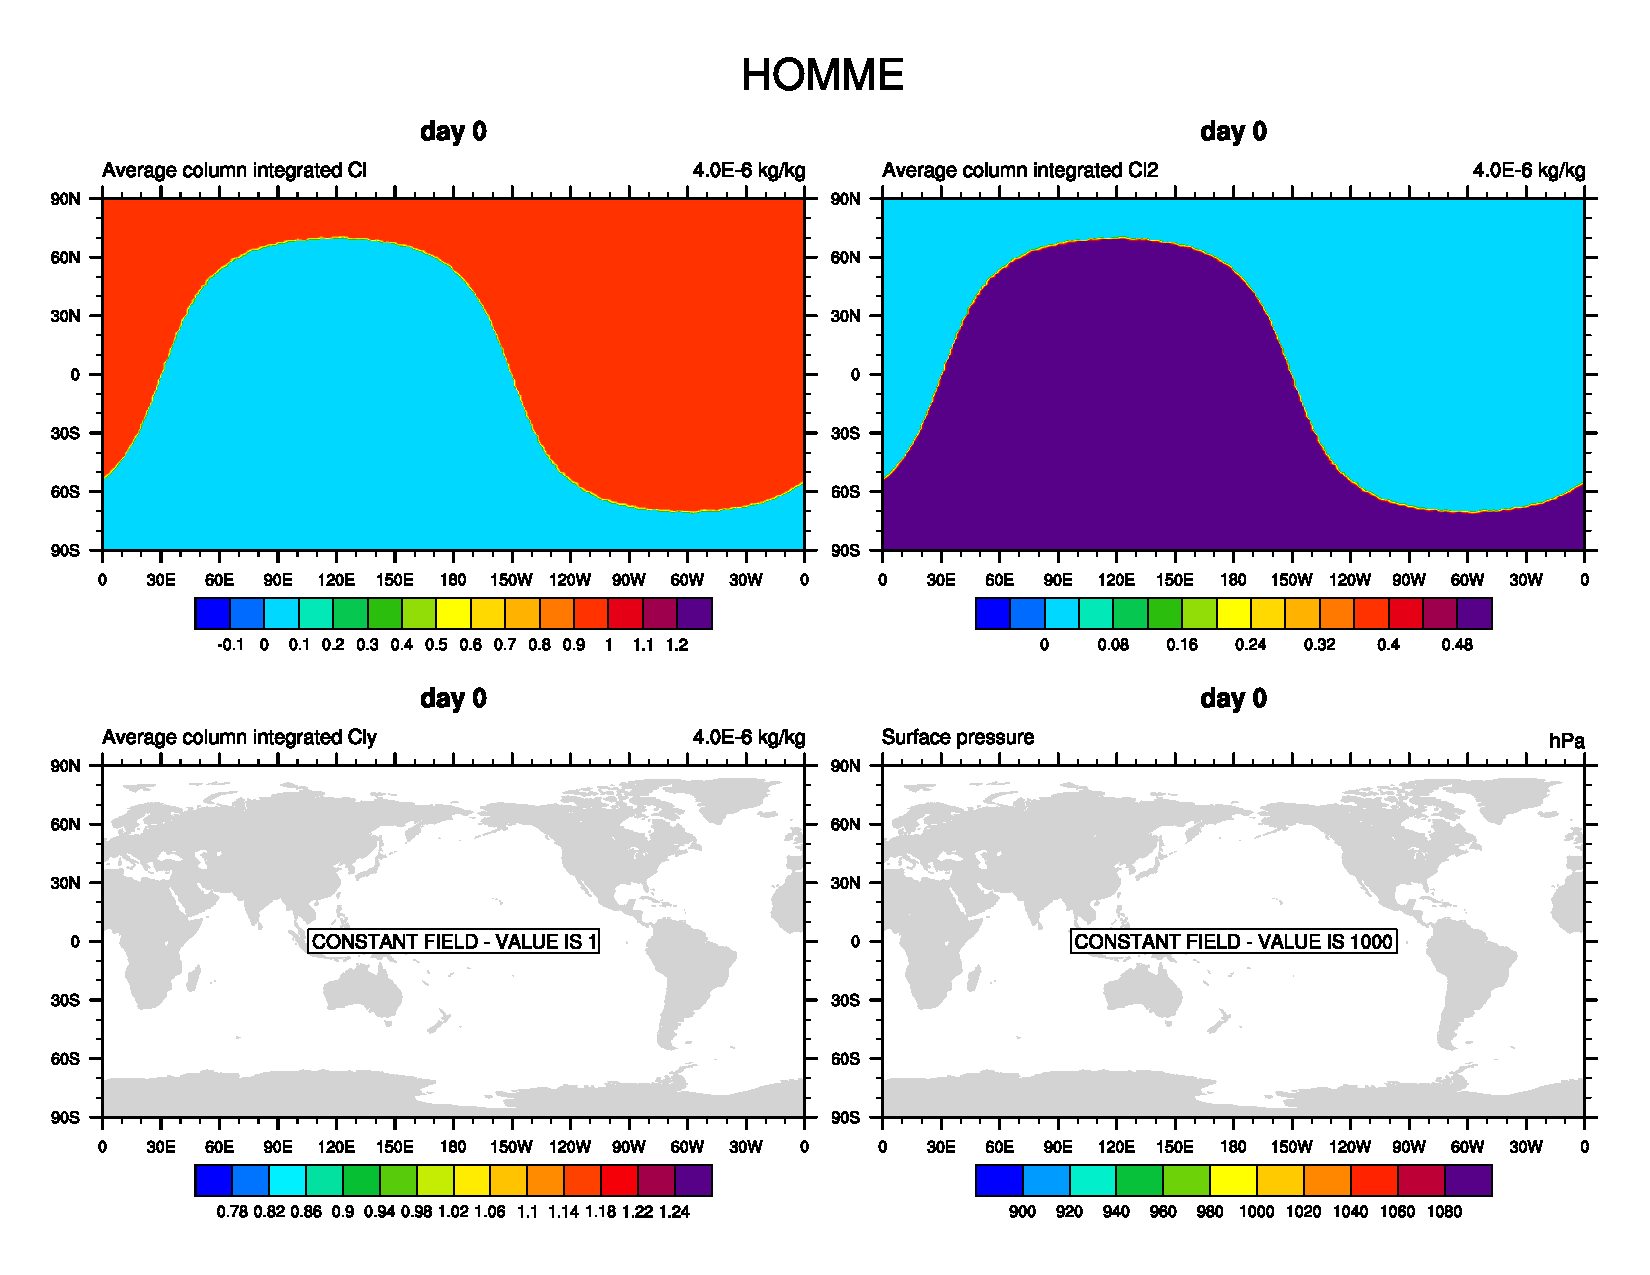
\includegraphics[width=\linewidth]{terminator-2d-se-day0.pdf}
\caption{Contour lines of $<q_{Cl}>/(4.0\times 10^{-6})$, (upper left), $<q_{Cl2}>/(4.0\times 10^{-6})$ (upper right), $<q_{Cly}>$ (lower left) and surface pressure (lower right) at day 0 (initial conditions).}
\label{fig:terminator-2d-se-day0}
\end{figure}
\begin{eqnarray}
q_{Cl}(\lambda,\theta,z,t=0)&=&D-r, \\
q_{Cl2}(\lambda,\theta,z,t=0)&=&\frac{1}{2}\left( q_{Cly} - D + r\right),
\end{eqnarray}
where $q_{Cly}=4.0\times 10^{-6}$kg/kg,
\begin{align}
 r &= \frac{k_1}{4 k_2}, \\
 D &= \sqrt{r^2 + 2 r q_{Cly}},
\end{align}
and reaction coefficients $k_1$ and $k_2$ are given in appendix \ref{sec:ToyChemistry} (equations \eqref{app:term_k1} and \eqref{app:term_k2}). 

The forcing terms are computed analytically (assuming no flow) over a (physics/chemistry) time-step $\Delta t$:
\begin{equation}
F_{Cl}^n= - L_{\Delta t} \frac{ (q_{Cl}^n - D + r ) (  {q_{Cl}}^n  + D + r  ) }{ 1+e^{-4 k_2 D \Delta t} + \Delta t L_{\Delta t} (q_{Cl}^n + r )  }.
\end{equation}
where $q_{Cl}^n$ is the value of $q_{Cl}$ at the beginning of the n'th time step and
\begin{equation}
  L_{\Delta t} = 
  \left\{ 
     \begin{array}{cc}  
          \frac{1-e^{-4 k_2 D \Delta t}}{D \Delta t}  &\mbox{if }  D > 0 \\[1ex]
          4k_2 &\mbox{if } D = 0.
      \end{array} 
   \right. \label{eq:linvsexp}
\end{equation}
and by conservation,
\begin{equation}
F_{\mathrm{Cl}_2  }^n = -\frac{1}{2} F_{\mathrm{Cl}  }^n .
\end{equation}
In implementation, $L_{\Delta t} $ needs some care.  As $4 k_2 D \Delta t$ approaches machine precision, it is useful to simply use the formula for $D=0$ rather than the expression for $D>0$. The chemistry/physics updated mixing ratios are given by
\begin{eqnarray}
q^n_{Cl}+\Delta t\, F_{Cl}^n,\\
q^n_{Cl2}+\Delta t\, F_{Cl2}^n.
\end{eqnarray}
In terms of Fortran code the analytical forcing is given by:
\begin{verbatim}
  ! dt is size of physics time step
  cly = cl + 2.0*cl2

  r = k1 / (4.0*k2)
  d = sqrt( r*r + 2.0*r*cly )
  e = exp( -4.0*k2*d*dt )

  if( abs(d*k2*dt) .gt. 1e-16 )
    el = (1.0-e) / (d*dt)
  else
    el = 4.0*k2
  endif

  f_cl  = -el * (cl-d+r) * (cl+d+r) / (1.0 + e + dt*el*(cl+r))
  f_cl2 = -f_cl / 2.0
\end{verbatim}
The reaction rates are defined by
\begin{verbatim}
  ! k1 and k2 are reaction rates
  k1_lat_center =  20.0 ! degrees
  k1_lon_center = 300.0 ! degrees
  k1 = max(0.d0,sin(lat)*sin(k1_lat_center) 
           + cos(lat)*cos(k1_lat_center)*cos(lon-k1_lon_center))
  k2 = 1.0
\end{verbatim}
The initial condition is defined by
\begin{verbatim}
  cly = 4.0e-6

  r = k1 / (4.0*k2)
  d = sqrt( r*r + 2.0*cly*r )

  cl = d-r
  cl2 = cly / 2.0 - (d-r) / 2.0
\end{verbatim}
Fortran subroutines that, given $(\lambda,\theta)$ will return the tendencies for $q_{Cl}$ (mixing ratio) and $q_{Cl2}$ (mixing ratio), are provided as supplemental material in \cite{LCLVT2015GMD}. Similarly for the forcing terms.

The `toy' terminator chemistry test here uses the baroclinic wave initialization (described in section \ref{sec:baroclinic_wave}) based on the moist setup and the flow will transport the two species that interact non-linearly with each other through the toy chemistry. A physics time-step of 30 minutes and 15 minutes, respectively, is used. Note that if the user has the baroclinic wave setup the only additional work is to initialize two tracers and implement the chemistry. Example solutions are shown for HOMME (High-Order Method Modeling Environment) \cite{DetAl2012IJHPCA} spectral elements and HOMME-CSLAM \cite{LetAl2016MWR}. The latter model is based on CSLAM \cite{LNU2010JCP} transport of tracers consistently coupled with spectral element dynamics.

\subsubsection{Diagnostics}
If the initial conditions for $q_{Cl}$ and $2q_{Cl2}$ add up to a constant (as is the case in this setup) then no matter how the individual species evolve the weighted sum $q_{Cly}=q_{Cl}+2q_{Cl2}$ should be constant in space and time. Hence the analytical solution for $q_{Cly}$ is known. The terminator chemistry preserves the linear relationship between $q_{Cl}$ and $q_{Cl2}$ so the only causes for this relationship to break are:
\begin{itemize}
\item the transport operator (usually the limiter/filter) does not exactly preserve linear relations, and/or,
\item physics-dynamics coupling breaks the relationship (see, e.g., Figure \ref{fig:terminator-diags}).
\end{itemize}
The following diagnostics are used in this test case:
\begin{itemize}
\item Average column integrated mixing ratio (two-dimensional variable):
\begin{equation}
<q>=\frac{\int_{z=0}^{z_{top}} q\, dz}{\int_{z=0}^{z_{top}} dz}.
\end{equation}
where $q=q_{Cl},q_{Cl2}$. The global integrals should be computed consistently with the numerical method (preferably `inline' in the source code on the native grid and not using interpolated data).
\item $\ell_2(t)$, $\ell_\infty(t)$ and relative mass change $\Delta M(t)$ error norms for Cl$_y$:
\begin{align}
\ell_2(t)&=\frac{\sqrt{\int_{z=0}^{z_{top}}\left(<q_{Cly}>-4.0\times 10^{-6}\right)^2 dz}}{\sqrt{\int_{z=0}^{z_{top}}\left(4.0\times 10^{-6}\right)^2 dz}},\\
\ell_\infty(t)&=\frac{\max_{\text{all }\lambda, \theta} |<q_{Cly}>-4.0\times 10^{-6}|}{4.0\times 10^{-6}},\\
\Delta M(t)&=\frac{\int_{z=0}^{z_{top}}q_{Cly}dz-M_0}{M_0}
\end{align}
respectively, where
\begin{equation}
<q_{Cly}>=<q_{Cl}+2q_{Cl2}>.
\end{equation}
and $M_0$ is the initial mass of Cl$_y$
\begin{equation}
M_0=\int_{z=0}^{z_{top}}4.0\times 10^{-6}dz.
\end{equation}
\end{itemize}
Note that if the physics-dynamics coupling procedure breaks $Cl_y$ conservation it can be very subtle but shows in the $\Delta M(t)$ diagnostic (see, e.g., Figure \ref{fig:terminator-diags}).
%\begin{equation}
%q_{Cly}=q_{Cl}+2q_{Cl2}.
%\end{equation}
%The exact solution is that $q_{Cly}$ remains constant in time:
%\begin{equation}
%q_{Cly}(t)=q_{Cly}(t=0)=4.0\times 10^{-6}\, kg/kg.
%\end{equation}






\begin{figure}[tb]
\center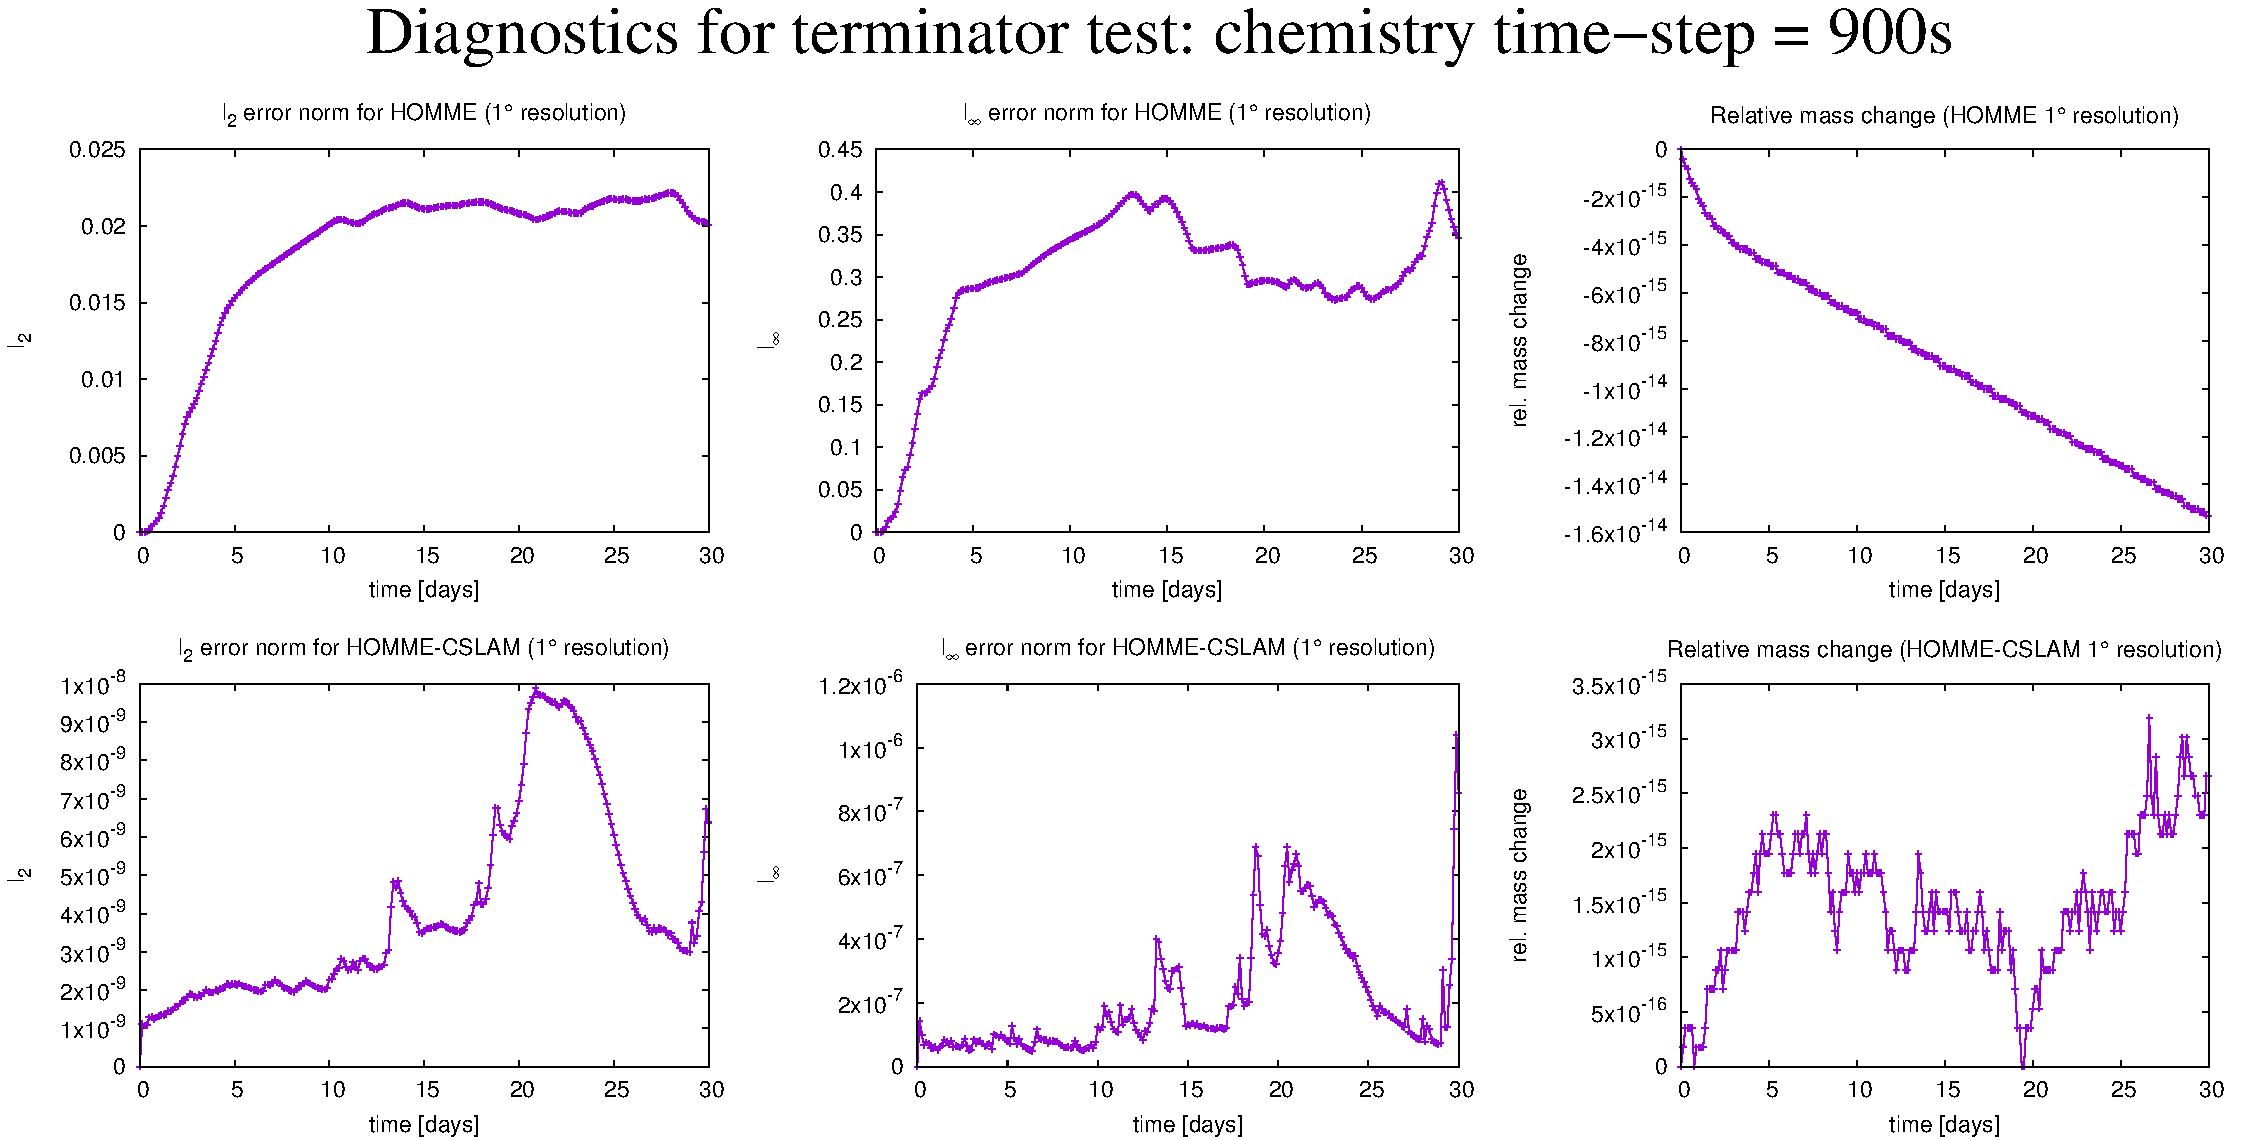
\includegraphics[width=\linewidth]{terminator_diags-t_phys900.pdf}
\center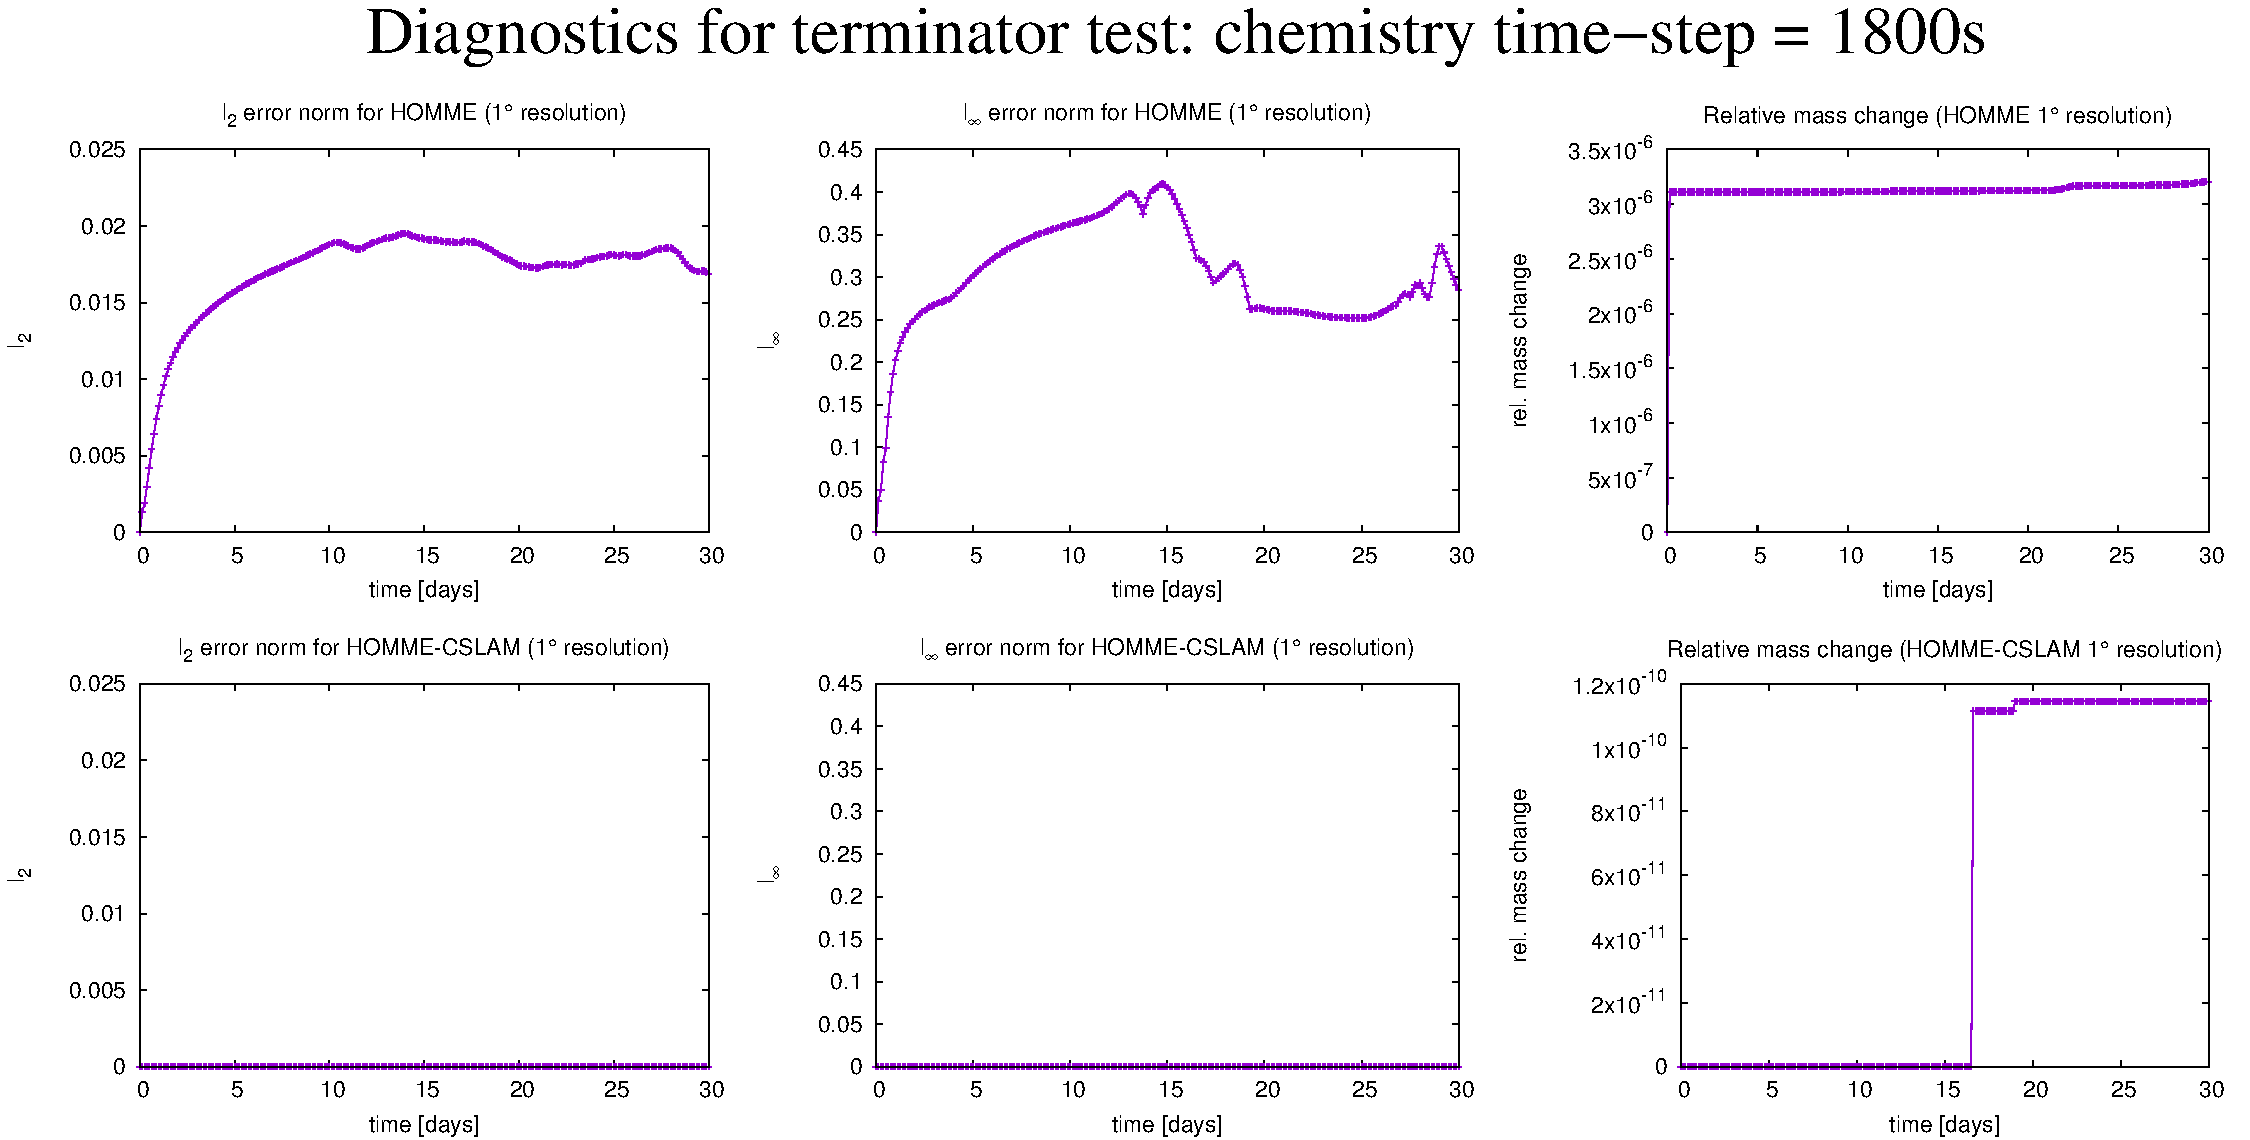
\includegraphics[width=\linewidth]{terminator_diags-t_phys1800.pdf}
  \caption{Global error norms $\ell_2(t)$ (column 1), $\ell_\infty(t)$ (column 2) and relative mass change $\Delta M(t)$ (column 3) for $q_{Cly}$ for HOMME  (row 1 and 3) and HOMME-CSLAM  (row 2 and 4) with physics/chemistry time-step of 15 minutes (row 1 and 2) and 30 minutes (row 3 and 4), respectively. The non-conservation of Cl$_y$ mass ($\Delta M(t)$) for physics time-step of 30 minutes is due to physics-dynamics coupling in which the tendencies are altered if they result in negative mixing ratios. For HOMME-CSLAM this happens at one point around day 16 and 18, respectively, whereas it happens frequently (in time and space) for HOMME.}\label{fig:terminator-diags}
\end{figure} 



%\cite{LCLVT2015GMD}
%\subsection{Grid spacings, simulation time, output and diagnostics}
%
%\begin{itemize}
%\item Dry simulations with the Toy Chemistry module (Appendix \ref{sec:ToyChemistry}) should be performed at 1$^\circ$ resolution with 30 vertical levels for 12 days.
%\item Plots of $q_{Cl}$, $q_{Cl2}$ and $q_T$ at 5000m altitude should be produced after $1$, $5$ and $12$ days. 
%\item Experiments could address the coupling frequency between the dynamics and physics.
%\end{itemize}




\subsection{Grid spacings, simulation time, output and diagnostics}

\begin{itemize}
\item Reference simulations (dry and moist) should be performed at 1$^\circ$ resolution with 30 vertical levels for 15 days.  Plots should be produced for the moist simulation and the anomaly between moist and dry simulations at day 9, 12 and 15.
\item Plots of minimum surface pressure over the duration of the simulation for both dry and moist configurations.
\item Experiments could address the coupling frequency between the dynamics and physics.
\item A variable resolution simulation should be performed that (a) studies the effect of the baroclinic wave transitioning from coarse resolution to fine resolution and (b) studies the effect of enhanced resolution near the front.
\item Terminator chemistry (use physics time-step of 30 minutes and 15 minutes): 
\begin{itemize}
\item Please plot contour lines for $<q_{Cl}>/(4.0\times 10^{-6})$ at day 9. Contour interval must be 0.1 with zero contour. Please offset the zero contour \verb+-1.0E-12+ to avoid contouring round-off undershoots. Contour levels used in Figure \ref{fig:terminator-2d-se} are\\
(\verb+-0.1,-1.0E-12,0.1,0.2,0.3,0.4,0.5,0.6,0.7,0.8,0.9,1.0,1.2+)
\item Please plot contour lines for $<q_{Cl2}>/(4.0\times 10^{-6})$ at day 9. Contour interval must be 0.04 with round-off offset zero contour.  Contour levels used in Figure \ref{fig:terminator-2d-se} are\\
(\verb+-0.04,-1.0E-12,0.04,0.08,0.12,0.16,0.20,0.24,0.28,+\\
\verb+0.32,0.36,0.40,0.44,0.48+)
\item Please plot contour lines for $<q_{Cly}>/(4.0\times 10^{-6})$ at day 9. Contour interval must be 0.04 (or 0.02 or 0.01 depending on your data) excluding the 1.0 contour but symmetric about 1.0. Contour levels used in Figure \ref{fig:terminator-2d-se} are\\
(\verb+0.78,0.82,0.86,0.90,0.94,0.98,1.02,1.06,1.1,1.14,1.18,1.22,1.24,+
\verb+1.08,1.12,1.16,1.20+)
\item Please plot global error norms $\ell_2(t)$, $\ell_\infty(t)$ and relative mass change $\Delta M(t)$ for $q_{Cly}$ as a function of time from day 0 to 30 preferably with 3 hourly time spacing. Use vertical axis adjusted to your data. See example on Figure \ref{fig:terminator-diags}.
\end{itemize}
\end{itemize}

\begin{figure}[t]
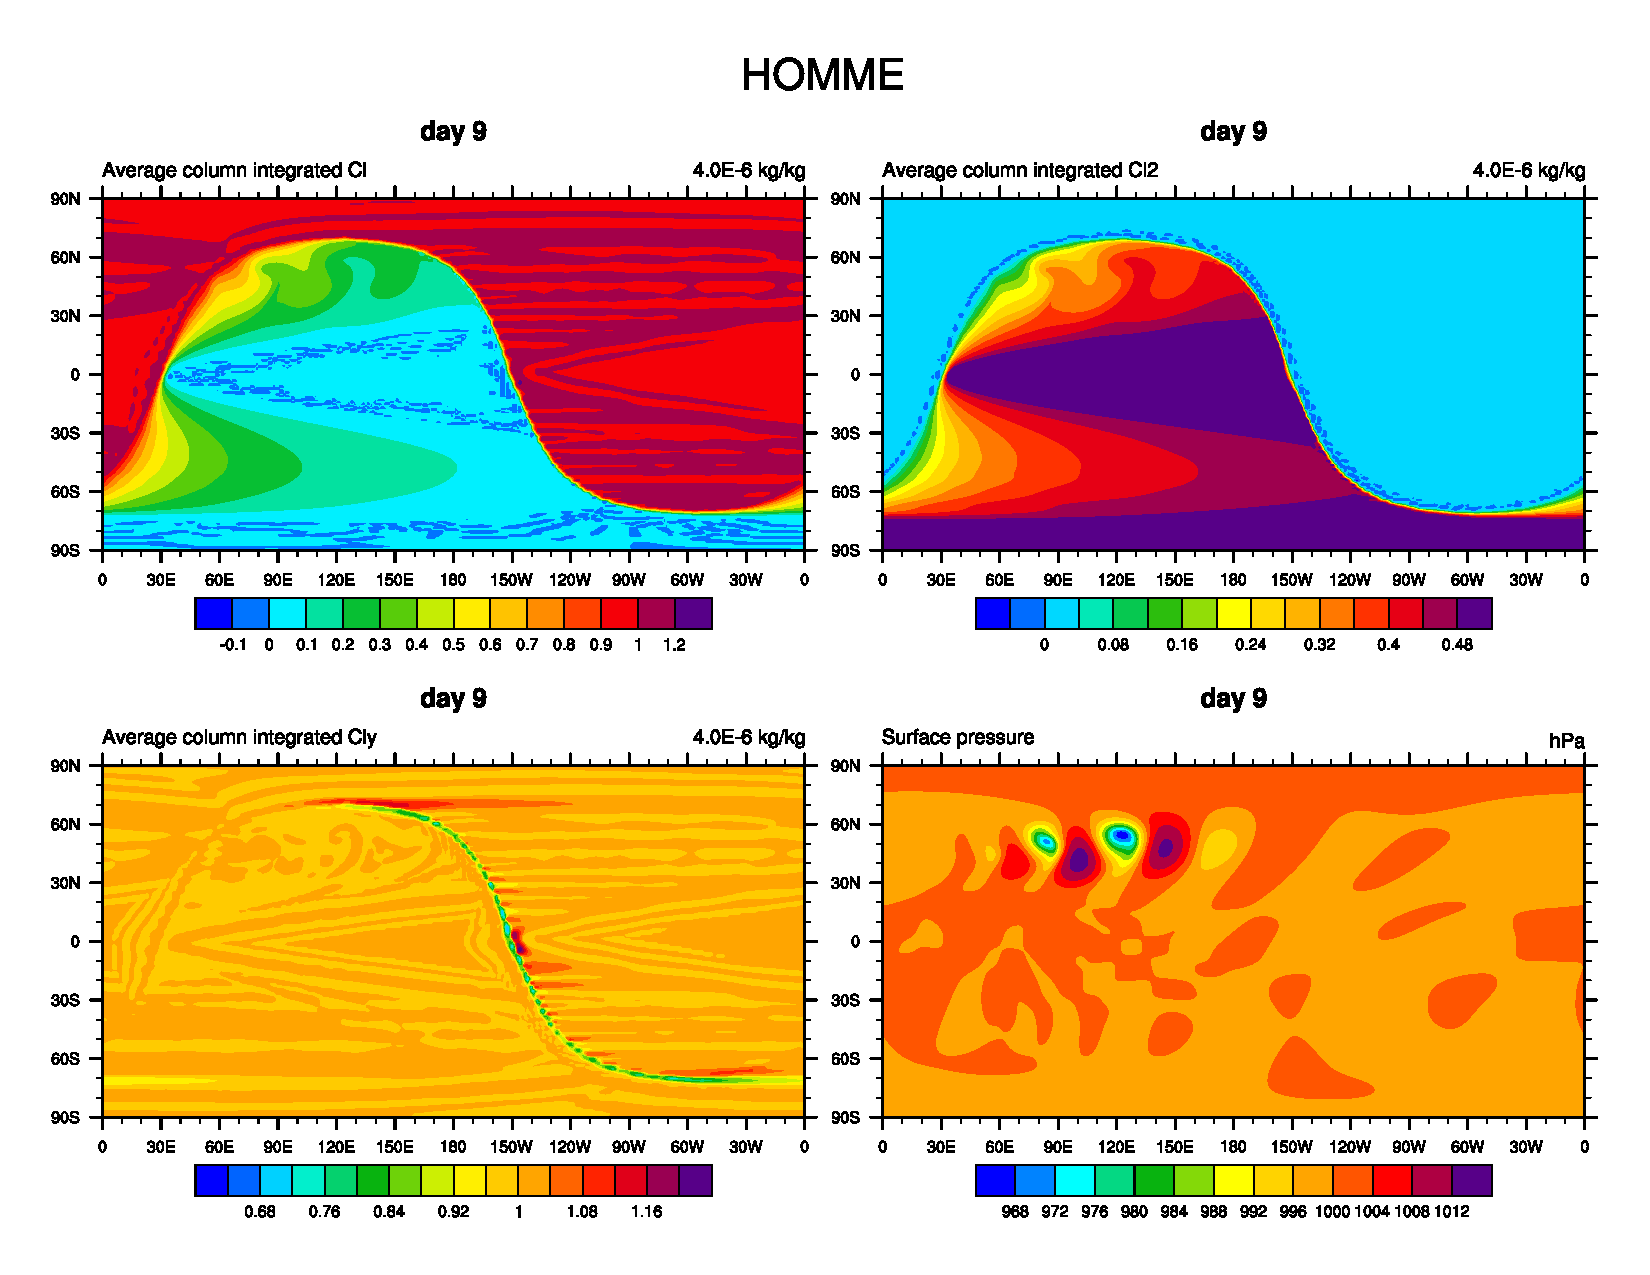
\includegraphics[width=0.9\linewidth]{terminator-2d-se-day9.pdf}
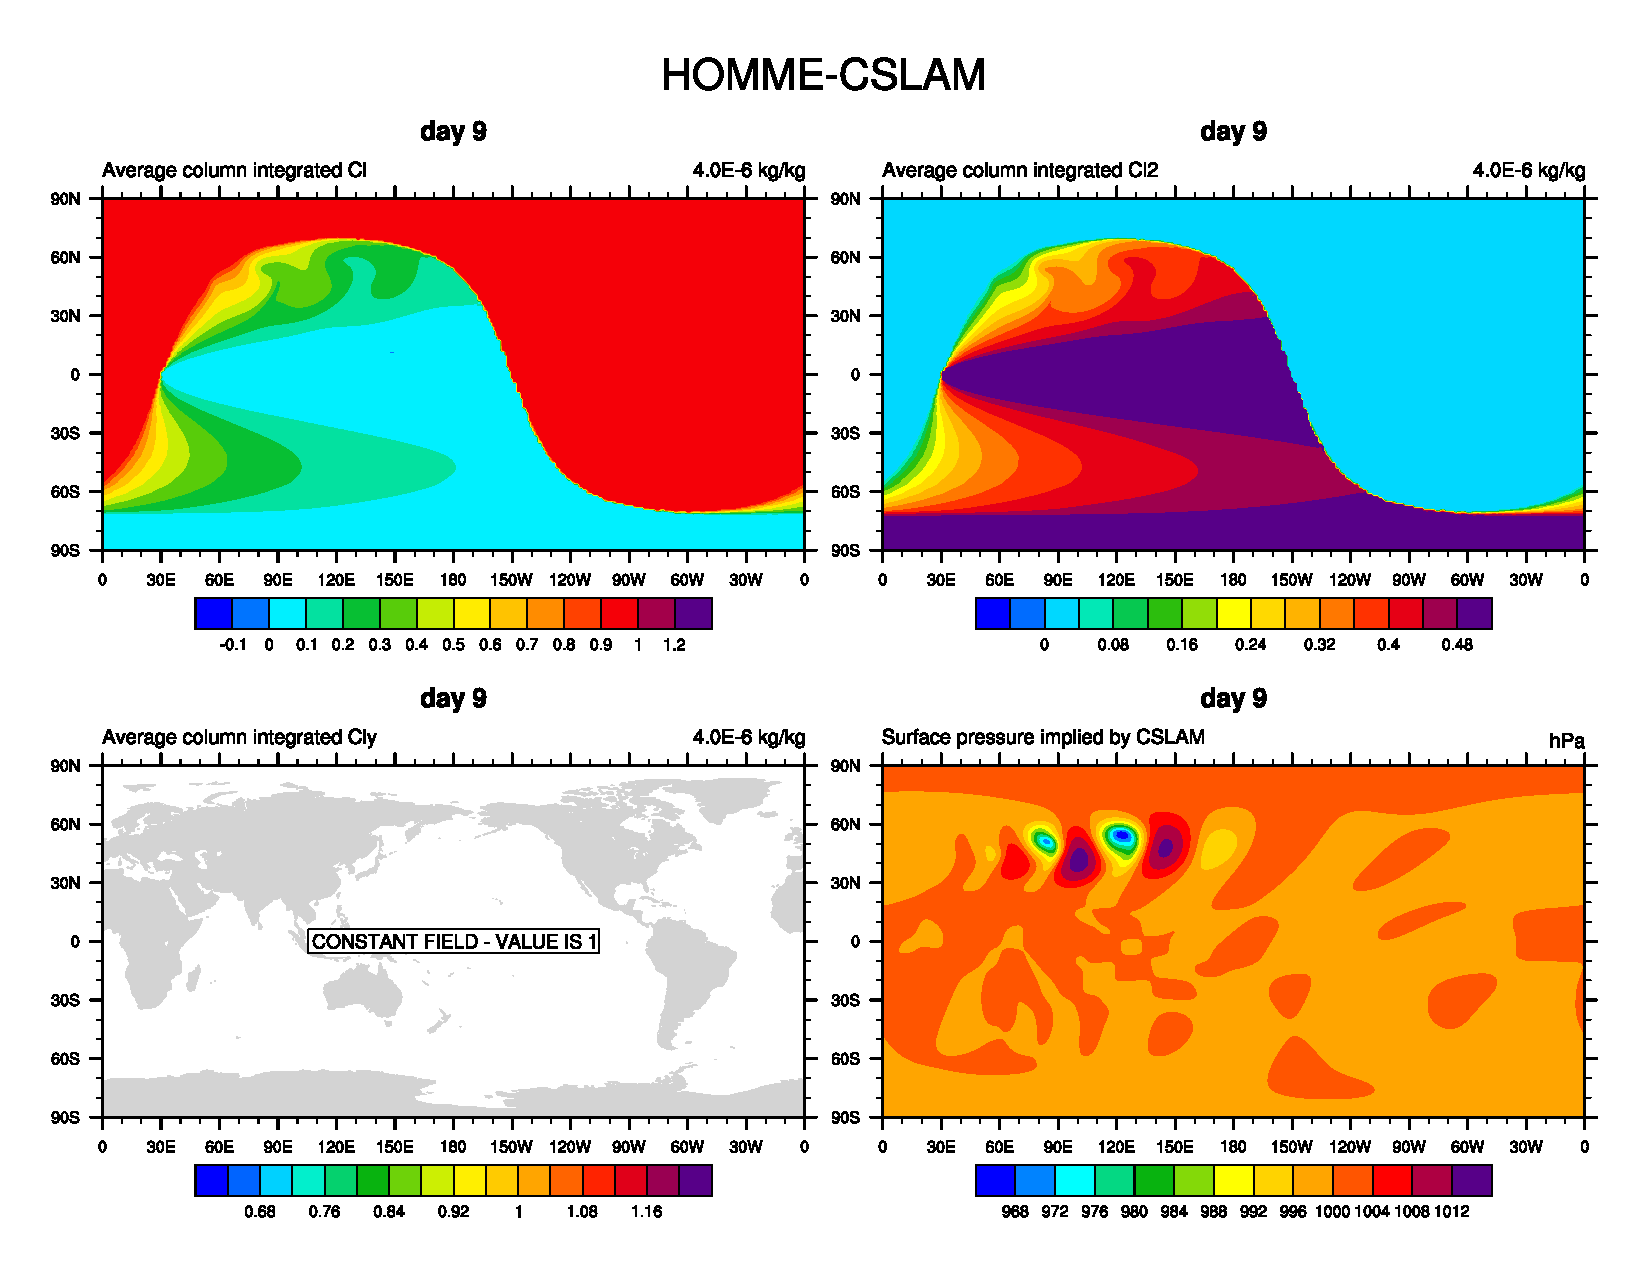
\includegraphics[width=0.9\linewidth]{terminator-2d-cslam-day9.pdf}
\caption{Upper panel of 4 plots is contour lines of $<q_{Cl}>/(4.0\times 10^{-6})$, (upper left), $<q_{Cl2}>/(4.0\times 10^{-6})$ (upper right), $<q_{Cly}>$ (lower left) and surface pressure (lower right) at day 9 simulated with HOMME at approximately $1^\circ$ resolution (30x30 elements on each cubed-sphere panel with 4x4 quadrature points in each element). Lower panel of 4 plots is the same as the upper panel but simulated with HOMME-CSLAM with 3x3 control volumes within each element. The results are based on the moist baroclinic wave setup (with no moist processes) and a physics-coupling time-step of 15 minutes.}
\label{fig:terminator-2d-se}
\end{figure}


\clearpage

\section{Tropical cyclone} \label{sec:tropical_cyclone}

The simplified tropical cyclone test case on a regular-size Earth is based on the work of \cite{reed2012idealized, reed2011analytic,reed2011impact, reed2011assessing}.  In this test an analytic vortex is initialized in a background environment which is tractable to a rapid intensification of tropical cyclones.  

\begin{table}[h]

\caption{List of constants used for the Ideaized Tropical Cyclone test}

\begin{tabular*}{\textwidth}{@{\extracolsep{\fill}}lll}
\hline Constant & Value & Description \\
\hline
$X$ & $1$ & small-planet scaling factor (regular-size Earth)\\
$z_t$ & $15000$ m & Tropopause height \\
$q_0$ & $0.021$ kg/kg & Maximum specific humidity amplitude \\
$q_t$ & $10^{-11}$ kg/kg & Specific humidity in the upper atmosphere \\
$T_0$ & $302.15$ K & Surface temperature of the air \\
$T_s$ & $302.15$ K & Sea surface temperature (SST), 29 C$^\circ$\\
$z_{q1}$ & $3000$ m & Height related to the linear decrease of $q$ with height \\
$z_{q2}$ & $8000$ m & Height related to the quadratic decrease of $q$ with height \\
$\Gamma$ & $0.007$\ K\ m$^{-1}$ & Virtual temperature lapse rate \\
$p_{b}$ & $1015$ hPa & Background surface pressure \\
$\varphi_c$ & $\pi / 18$ & Initial latitude of vortex center (radians) \\
$\lambda_c$ & $\pi$ & Initial longitude of vortex center (radians) \\
$\Delta p$ & $11.15$ hPa & Pressure perturbation at vortex center \\
$r_p$ & $282000$ m & Horizontal half-width of pressure perturbation \\
$z_p$ & $7000$ m & Height related to the vertical decay rate of $p$ perturbation \\
$\epsilon$ & $10^{-25}$ & Small threshold value \\
\hline 
\end{tabular*}

\end{table}

\subsection{Initialization}

The background state consists of a prescribed specific humidity profile, virtual temperature and pressure profile.  The initial profile is defined to be in approximate gradient wind balance.  The vertical sounding is chosen to roughly match an observed tropical sounding documented in \cite{jordan1958mean}.  The background specific humidity profile $\overline{q}(z)$ as a function of height $z$ is

\begin{equation}
\begin{split}
\overline{q}(z)&=q_0 \exp\left(- \frac{z}{z_{q1}}\right)\exp\left[-\left(\frac{z}{z_{q2}}\right)^2\right] \text{ ~~for   } 0 \leq z \leq z_t \\
\overline{q}(z)&=q_t  \text{ ~~for   }  z_t \leq z
\end{split}
\end{equation}

The background virtual temperature sounding $\overline{T}_v(z)$ is split into two different representations for the lower and upper atmosphere.  It is given by
\begin{equation}
\begin{array}{ll} \label{eq:tc_virtualtemperaturebg}
%\phantom{T_{vt} = }\overline{T}_v(z) = T_{v0} - \Gamma z & \mbox{for} \; 0 \le z \le z_t, \\
\overline{T}_v(z) = T_{v0} - \Gamma z & \mbox{for} \; 0 \le z \le z_t, \\
\overline{T}_v(z) = T_{vt} = T_{v0} - \Gamma z_t & \mbox{for} \; z_t < z, 
\end{array}
\end{equation} with the virtual temperature at the surface $T_{v0}$ = $T_0 (1+0.608 \, q_0)$ and the virtual temperature at the tropopause level $T_{vt}$ = $T_{v0} - \Gamma z_t$.  The background temperature profile can be obtained from (\ref{eq:virtualtemperature}).

The background vertical pressure profile $\overline{p}(z)$ of the moist air is computed using the hydrostatic balance and (\ref{eq:tc_virtualtemperaturebg}). The profile is given by:
\begin{equation}
\begin{array}{ll}\label{eq4}
\displaystyle \overline{p}(z) = p_b \left( \frac{T_{v0} - \Gamma z}{T_{v0}} \right )^{g / R_d \Gamma} & \mbox{for} \; 0 \le z \le z_t, \\
\displaystyle \overline{p}(z) = p_t \, \exp{\left(\frac{g (z_t - z)}{R_d T_{vt}} \right)} & \mbox{for} \; z_t < z.
\end{array}
\end{equation}  The pressure at the tropopause level $z_t$ is continuous and given by 
\begin{equation}\label{eq4.5}
p_t = p_b \left( \frac{T_{vt}}{T_{v0}} \right )^{\frac{g}{R_d \Gamma}},
\end{equation}
which, for the given set of parameters, is approximately 130.5 hPa. 

\subsubsection{Axisymmetric Vortex}

The pressure equation $p(r,z)$ for the moist air is comprised of the background pressure profile (\ref{eq4}) plus a 2D pressure perturbation $p'(r,z)$,
\begin{equation} \label{eq5}
p(r,z) = \overline{p}(z) + p^\prime(r,z),
\end{equation} where $r$ symbolizes the radial distance (or radius) to the center of the prescribed vortex.  On the sphere $r$ is defined using the great circle distance
\begin{equation}
r = a \arccos{ \left ( \sin{\varphi_c} \, \sin{\varphi} + \cos{\varphi_c} \, \cos{\varphi} \, \cos{(\lambda - \lambda_c)} \right )}.
\end{equation}  The perturbation pressure is defined as
\begin{align} \label{test5:p_pert}
p^\prime(r,z) & = -\Delta p \, \exp\left[{-\left (\frac{r}{r_p} \right ) ^{3/2}} {-\left (\frac{z}{z_p} \right ) ^{2}}\right] \left ( \frac{T_{v0} - \Gamma z}{T_{v0}} \right )^{\frac{g}{R_d \Gamma}} & & \mbox{for $\; 0 \le z \le z_t$},  \nonumber \\
p^\prime(r,z) & = 0 & & \mbox{for} \; z_t < z.
\end{align}  The pressure perturbation depends on the pressure difference $\Delta p$ between the background surface pressure $p_b$ and the pressure at the center of the initial vortex, the pressure change in the radial direction $r_p$ and the pressure decay with height within the vortex $z_p$.  The moist surface pressure $p_s(r)$ is computed by setting $z = 0$ m in (\ref{eq5}), which gives
\begin{equation}
\label{eq:ps}
p_s(r) = p_b - \Delta p \, \exp\left[{-\left (\frac{r}{r_p} \right ) ^{3/2}}\right].
\end{equation}

The axisymmetric virtual temperature $T_v(r,z)$ is computed using the hydrostatic equation and ideal gas law
\begin{equation}
T_v(r,z) = -\frac{g p(r,z)}{R_d} \left( \frac{\partial p(r,z)}{ \partial z} \right)^{-1}.
\end{equation}  Again it can be written as a sum of the background state and a perturbation,
\begin{equation} \label{eq:virt_temp}
T_v(r,z) = \overline{T}_v(z) + T_v^\prime(r,z),
\end{equation} where the virtual temperature perturbation is defined as
\begin{align}
\label{eq:Tv}
T_v^\prime(r,z) &= (T_{v0} - \Gamma z ) \left\{ \left [1+ \frac{2R_d(T_{v0} - \Gamma z)z}{gz_p^2 \left[ 1 - \frac{p_b}{\Delta p}\exp\left({\left (\frac{r}{r_p} \right ) ^{3/2}} + {\left (\frac{z}{z_p} \right ) ^{2}} \right) \right] }\right]^{-1} - 1 \right\} & & \mbox{for} \; 0 \le z \le z_t, \nonumber \\
T_v^\prime(r,z) &= 0 & & \mbox{for} \; z_t < z.
\end{align} 

The axisymmetric specific humidity $q(r,z)$ is set to the background profile everywhere
\begin{eqnarray}
\label{eq:q}
q(r,z) = \overline{q}(z).
\end{eqnarray}  Consequently, the temperature can be written as
\begin{equation} \label{test5:T_eqn}
T(r,z) = \overline{T}(z) + T^\prime(r,z),
\end{equation} with the temperature perturbation
\begin{align} \label{eq:temperature}
T^\prime(r,z) &= \frac{T_{v0} - \Gamma z}{1+0.608\overline{q}(z)} \left\{ \left [1+ \frac{2R_d(T_{v0} - \Gamma z)z}{gz_p^2 \left[ 1 - \frac{p_b}{\Delta p}\exp\left({\left (\frac{r}{r_p} \right ) ^{3/2}} + {\left (\frac{z}{z_p} \right ) ^{2}} \right) \right] }\right]^{-1} - 1 \right\} & & \mbox{for} \; 0 \le z \le z_t, \nonumber \\
T^\prime(r,z) &= 0 & & \mbox{for} \; z_t < z. 
\end{align}  
Due to the small specific humidity value in the upper atmosphere (10$^{-11}$ kg/kg for $z > z_t$) the virtual temperature equals the temperature to a very good approximation in this region. The formulation presented here is equivalent to the one presented in \cite{reed2012idealized}.

If the density of the moist air needs to be initialized its formulation is based on the ideal gas law
\begin{equation} \label{eq:density}
\rho(r,z) = \frac{p(r,z)}{R_d T_v(r,z)}
\end{equation} 
which utilizes the moist pressure (\ref{eq5}) and virtual temperature (\ref{eq:virt_temp}). The surface elevation $z_s$ and thereby the surface geopotential $\Phi_s=g z_s$ are set to zero.
 
Finally, the tangential velocity field $v_T(r,z)$ of the axisymmetric vortex is defined by utilizing the gradient-wind balance, which depends on the pressure (\ref{eq5}) and the virtual temperature (\ref{eq:Tv}). The tangential velocity is given by
\begin{eqnarray}
\label{eq:gradient-wind}
v_T(r,z) = -\frac{f_cr}{2}+\sqrt{ \frac{f_c^2r^2}{4}+\frac{R_d \, T_v(r,z) \, r}{p(r,z)} \frac{\partial p(r,z)}{\partial r}},
\end{eqnarray}
where $f_c = 2 \Omega \sin(\varphi_c)$ is the Coriolis parameter at the constant latitude $\varphi_c$. Substituting $T_v(r,z)$ and $p(r,z)$ into ({\ref{eq:gradient-wind}) gives
\begin{align}
\label{eq:gradient-wind-expr}
v_T(r,z) & = -\frac{f_cr}{2}+\sqrt{ \frac{f_c^2r^2}{4}-\frac{\frac{3}{2} \left( \frac{r}{r_p}\right)^{3/2} (T_{v0}-\Gamma z) R_d}{1+\frac{2R_d(T_{v0}-\Gamma z)z}{g z_p^2}-\frac{p_b}{\Delta p}\exp\left({\left (\frac{r}{r_p} \right ) ^{3/2}} + {\left (\frac{z}{z_p} \right ) ^{2}} \right)}} & & \mbox{for} \; 0 \le z \le z_t, \nonumber \\
v_T(r,z) & = 0 & & \mbox{for} \; z_t < z.
\end{align}  The last step is to split the tangential velocity (\ref{eq:gradient-wind-expr}) into its zonal and meridional wind components $u(\lambda,\varphi,z)$ and $v(\lambda,\varphi,z)$. Similar to \cite{nair2008moving} these are computed using the following expressions,
\begin{eqnarray}
d_1 &=& \sin\varphi_c \, \cos\varphi - \cos\varphi_c \, \sin\varphi \, \cos(\lambda-\lambda_c) \\
d_2 &=& \cos\varphi_c \, \sin(\lambda-\lambda_c) \\
d &=& \max \big({\epsilon,\sqrt{ {d_1}^2 + {d_2}^2} } \big),
\end{eqnarray}
which are utilized in the projections
\begin{eqnarray}
\label{eqn:u_wind}
u(\lambda,\varphi,z) &=& \frac{v_T(\lambda,\varphi,z) \, d_1}{d}\\ \label{eqn:v_wind}
v(\lambda,\varphi,z) &=& \frac{v_T(\lambda,\varphi,z) \, d_2}{d} \,.
\end{eqnarray}
A small $\epsilon = 10^{-25}$ value avoids divisions by zero.  The vertical velocity is set to zero.

\subsection{Grid spacings, simulation time, output and diagnostics}

\begin{itemize}
\item Moist simulations should be performed at 0.5$^\circ$ resolution with 30 vertical levels for 10 days.
\item Plots of minimum surface pressure over the duration of the simulation.
\item Experiments could address the coupling frequency between the dynamics and physics.
\item A variable resolution simulation should be performed that (a) studies the effect of the tropical cyclone transitioning from fine resolution to coarse resolution and (b) high resolution simulations down to 0.125$^\circ$ over the tropical cyclone.
\end{itemize}


\clearpage

\section{Mesoscale Storm}  \label{sec:mesoscale_storm}

The mesoscale storm test permits the study of a non-hydrostatic moist feature with strong vertical velocities and associated precipitation and is based on the work of \cite{klemp1978simulation}.

\begin{table}[h]

\caption{List of constants used for the Mesoscale Storm test}

\begin{tabular*}{\textwidth}{@{\extracolsep{\fill}}lll}
\hline Constant & Value & Description \\
\hline
$X$ & $120$ & Small-planet scaling factor (reduced Earth)\\
$\theta_{tr}$ & $343$ K & Temperature at the tropopause \\
$\theta_0$ & $300$ K & Temperature at the equatorial surface \\
$z_{tr}$ & $12000$ m & Altitude of the tropopause \\
$T_{tr}$ & $213$ K & Temperature at the tropopause \\
$U_s$ & $30$ m/s & Maximum zonal wind velocity \\
$U_c$ & $15$ m/s & Coordinate reference velocity \\
$z_{s}$ & $5000$ m & Lower altitude of maximum velocity \\
$\Delta z_{u}$ & $1000$ m & Transition distance of velocity \\
$\Delta \theta$ & $3$ K & Thermal perturbation magnitude \\
$\lambda_p$ & $0$ & Thermal perturbation longitude \\
$\varphi_p$ & $0$ & Thermal perturbation latitude \\
$r_p$ & $X \times 10000$ m & Perturbation horizontal half-width \\
$z_{c}$ & $1500$ m & Perturbation center altitude \\
$z_{p}$ & $1500$ m & Perturbation vertical half-width \\
\hline 
\end{tabular*}

\end{table}

It is assumed that the saturation mixing ratio is given by
\begin{equation}
q_{vs}(p,T) = \left( \frac{380.0}{p} \right) \exp\left(17.27 \times \frac{T-273.0}{T-36.0}\right)
\end {equation}  The definition of this test case relies on hydrostatic and gradient wind balance, written in terms of Exner pressure $\pi$ and virtual potential temperature $\theta_v$ as
\begin{equation} \label{eq:BalanceEq}
\pdiff{\pi}{z} = - \frac{g}{c_p \theta_v}, \quad \mbox{and} \quad u^2 \tan \varphi = - c_p \theta_v \pdiff{\pi}{\varphi}.
\end{equation}  These equations can be combined to eliminate $\pi$, leading to
\begin{equation} \label{eq:CombinedBalanceEq}
\pdiff{\theta_v}{\varphi} = \frac{\sin (2 \varphi)}{2 g} \left( u^2 \pdiff{\theta_v}{z} - \theta_v \pdiff{u^2}{z} \right).
\end{equation}

The wind velocity is analytically defined throughout the domain.  Meridional and vertical wind is initially set to zero.  The zonal wind is obtained from
\begin{equation}
\overline{u}(\varphi,z) = \left\{ \begin{array}{ll}
\displaystyle \left(U_s\frac{z}{z_t}-U_c\right)\cos(\varphi) & \mbox{for $z < z_s - \Delta z_u$}, \\[2.0ex]
\displaystyle \left(-\frac{4}{5}+3\frac{z}{z_s}-\frac{5}{4}\frac{z^2}{z_s^2}\right)U_s-U_c & \mbox{for $\vert z-z_s \vert \leq \Delta z_u$} \\[2.0ex]
\displaystyle \left(U_s-U_c\right)\cos(\varphi) & \mbox{for $z > z_s + \Delta z_u$}
\end{array} \right.
\end{equation}

The equatorial profile is determined through numerical iteration.  Potential temperature at the equator is specified via
\begin{equation}
\theta_{\text{eq}}(z) = \left\{ \begin{array}{ll} \displaystyle \theta_0 + (\theta_{tr} - \theta_0)\left(\frac{z}{z_{tr}}\right)^{\frac{5}{4}}  & \mbox{for $0 \leq z \leq z_{tr}$,} \\[2.0ex]
\displaystyle \theta_{tr} \exp\left(-\frac{g(z-z_{tr})}{c_pT_{tr}}\right) & \mbox{for $z_{tr} \leq z$} \end{array} \right.
\end{equation}  And relative humidity is given by
\begin{equation}
\overline{H}(z) = \left\{ \begin{array}{ll} \displaystyle 1 + \frac{3}{4}\left(\frac{z}{z_{tr}}\right)^{5/4} & \mbox{for $0 \leq z \leq z_{tr}$,} \\[2.0ex]
\displaystyle \frac{1}{4} & \mbox{for $z_{tr} \leq z$.} \end{array} \right.
\end{equation}  Pressure and temperature at the equator are obtained by iterating on hydrostatic balance  with initial state
\begin{equation}
\theta_{v,\text{eq}}^{(0)}(z) = \theta_{\text{eq}}(z),
\end{equation} and iteration procedure
\begin{align}
\pi_{\text{eq}}^{(i)} &= 1 - \int_{0}^{z} \frac{g}{c_p \theta_{v,\text{eq}}^{(i)}} dz \\
p_{\text{eq}}^{(i)} &= p_0 (\pi^{(i)})^{c_p / R_d} \\
T_{\text{eq}}^{(i)} &= \theta_{\text{eq}}(z) \pi_{\text{eq}}^{(i)} \\
q^{(i)}_{\text{eq}} &= H(z) q_{vs}(p_{\text{eq}}^{(i)}, T_{\text{eq}}^{(i)}) \\
\theta_{v,\text{eq}}^{(i+1)} &= \theta_{\text{eq}}(z) (1 + M_v q^{(i)}_{\text{eq}})
\end{align}  This iteration procedure appears to converge to machine epsilon after approximately 10 iterations.  The equatorial moisture profile is then extended through the entire domain,
\begin{equation}
q(z, \varphi) = q_{\text{eq}}(z).
\end{equation}

Once the equatorial profile has been constructed, the virtual potential temperature through the remainder of the domain can be computed by iterating on (\ref{eq:CombinedBalanceEq}),
\begin{align}
\theta_v^{(i+1)}(z,\varphi) = \theta_{v,\text{eq}}(z) + \int_{0}^{\varphi} \frac{\sin(2 \phi)}{2 g} \left(\overline{u}^2 \pdiff{\theta_{v}^{(i)}}{z} - \theta_v^{(i)} \pdiff{\overline{u}^2}{z} \right) d\varphi.
\end{align}  Again, approximately 10 iterations are needed for convergence to machine epsilon.  Once virtual potential temperature has been computed throughout the domain, Exner pressure throughout the domain can be obtained from (\ref{eq:BalanceEq}),
\begin{equation}
\pi(z,\varphi) = \pi_{eq}(z) - \int_{0}^{\varphi} \frac{u^2 \tan \varphi}{c_p \theta_v} d\varphi,
\end{equation} and so
\begin{align}
p(z,\varphi) &= p_0 \pi(z,\varphi)^{c_p / R_d}, \\
T_v(z,\varphi) &= \theta_v(z,\varphi) (p / p_0)^{R_d / c_p}.
\end{align}

\subsection{Potential temperature perturbation}

To initiate convection, a thermal perturbation is introduced in the initial potential temperature field:
\begin{equation}
\theta^\prime(\lambda,\phi,z) = \left\{ \begin{array}{ll} \displaystyle \Delta \theta \cos^2\left(\frac{\pi}{2}R_{\theta}(\lambda, \varphi, z)\right) & \mbox{for $R_{\theta}(\lambda, \varphi, z) < 1$,} \\[2.0ex]
0 & \mbox{for $R_{\theta}(\lambda, \varphi, z) \geq 1$,} \end{array} \right.
\end{equation} where
\begin{equation}
R_{\theta}(\lambda, \varphi, z) = \left[ \left( \frac{R_c(\lambda, \varphi; \lambda_p, \varphi_p)}{r_p} \right)^2 + \left( \frac{z - z_c}{z_p} \right)^2 \right]^{1/2}.
\end{equation}

\subsection{Grid spacings, simulation time, output and diagnostics}

\begin{itemize}
\item Moist simulations should be performed at 1$^\circ$ resolution with 30 vertical levels for 2 hours.
\item Plots of vertical velocity and rainwater should be produced at 5 km altitude after 30, 60, 90 and 120 minutes over the domain $[0, 130E] \times [40S, 40N]$.
\item A plot of maximum vertical velocity over the duration of the simulation should be produced.
\item Experiments could address the coupling frequency between the dynamics and physics.
\item A variable resolution simulation should be performed that (a) studies the effect of the mesoscale storm transitioning from fine resolution to coarse resolution and (b) high resolution simulations down to 0.125$^\circ$ over the mesoscale storm.
\end{itemize}



%%%%%%%%%%%%%%%%%%%%%%%%%%%%%%%%%%%%%%%%%%%%%%%%%%%%%%%%%%%%%%%%%%%%%%%%%%%%%%%%%%%%%%%%%%%%%%%%%%%%%%%%%%%%%%%%%%%%%%%%%%%%%%%%%%

\bibliographystyle{wileyj}
\bibliography{DCMIP2016}

\begin{appendix}

%%%%%%%%%%%%%%%%%%%%%%%%%%%%%%%%%%%%%%%%%%%%%%%%%%%%%%%%%%%%%%%%%%%%%%%%%%%%%%%%%%%%%%%%%%%%%%%%%%%%%%%%%%%%%%%%%%%%%%%%%%%%%%%%%%

\section{Kessler Physics} \label{sec:KesslerPhysics}

The cloud microphysics update according to the following equation set:
\begin{alignat}{5}
\frac{\Delta \theta}{\Delta t} = & - \frac{L}{c_p \pi} & \Big( \frac{\Delta q_{vs}}{\Delta t} & + E_r  \Big) & \\
\frac{\Delta q_v}{\Delta t} = & & \frac{\Delta q_{vs}}{\Delta t} & + E_r \\
\frac{\Delta q_c}{\Delta t} = & & - \frac{\Delta q_{vs}}{\Delta t} & & - A_r & - C_r \\
\frac{\Delta q_r}{\Delta t} = & & & - E_r & + A_r & + C_r & - V_r \pdiff{q_r}{z},
\end{alignat} where $L$ is the latent heat of condensation, $A_r$ is the autoconversion rate of cloud water to rain water, $C_r$ is the collection rate of rain water, $E_r$ is the rain water evaporation rate, and $V_r$ is the rain water terminal velocity.

The pressure follows from the equation of state
\begin{equation}
p=\rho R_dT(1+0.61q_v)
\end{equation} with $p$ the pressure, $\rho$ the density of moist air, $R_d$ the gas constant for dry air, $T$ the temperature and $q_v$ the mixing ratio of water vapor. The equation is rewritten as a nondimensional pressure $\Pi$ equation.
\begin{equation}
\pi = \left(\frac{p}{p_0}\right)^{\frac{R_dT}{cp}}
\end{equation}

To determine the saturation vapor mixing ratio the Teten's formula is used,
\begin{equation}
q_{vs}(p,T) = \left( \frac{380.0}{p} \right) \exp\left(17.27 \times \frac{T-273.0}{T-36.0}\right)
\end {equation}

The autoconvection rate ($A_r$) and collection rate ($C_r$) follow Kessler parametrization and are defined by:
\begin{align}
A_r &= k_1(q_c-a) \\
C_r &= k_2q_cq_r^{0.875}
\end{align} With $k_1=0.001 \text{s}^{-1}$, $a=0.001 \text{g}.\text{g}^{-1}$ and $k_2=2.2 \text{s}^{-1}$ 

Deriving from \cite{klemp1978simulation} description of cloud water,rain water and water vapor mixing ratios. they are define as followed:
\begin{equation}
q_c^{n+1}=\mbox{max}(q_c^r-\Delta q_r,0)
\end{equation}
\begin{equation}
q_r^{n+1}=\mbox{max}(q_r^r-\Delta q_r+S,0)
\end{equation} where $S$ is the sedimentation term and $\Delta q_r$ is defined as
\begin{equation}
\Delta q_r=q_c^n-\frac{q_c^n-\Delta \text{t}\ \mbox{max}(A_r,0)}{1+\Delta \text{t} C_r}
\end{equation}

The Rain evaporation equation is defined similarly to \cite{ogura1971numerical} description:
\begin{equation}
E_r=\frac{1}{\rho}\frac{\left(1-\frac{q_v}{q_{vs}}\right)C(\rho q_r)^{0.525}}{5.4\times10^5+\frac{2.55\times10^6}{pq_{vs}}}
\end{equation}  With ventilation factor C define as 
\begin{equation}
C_r=1.6+124.9(\rho q_r)^{0.2046}
\label{venti}
\end{equation}

The liquid water terminal velocity is similar to \cite{soong1973comparison} description with a mean density adjustment as suggested by \cite{kessler1969distribution}:
\begin{equation}
V_r = 36349(\rho q_r)^{0.1346}\left(\frac{\rho}{\rho_0}\right)^{-\frac{1}{2}}
\end{equation}

%%%%%%%%%%%%%%%%%%%%%%%%%%%%%%%%%%%%%%%%%%%%%%%%%%%%%%%%%%%%%%%%%%%%%%%%%%%%%%%%%%%%%%%%%%%%%%%%%%%%%%%%%%%%%%%%%%%%%%%%%%%%%%%%%%

\section{`Toy' Chemistry} \label{sec:ToyChemistry}

The toy chemistry module represents a simple photolysis-driven chemical reaction that incorporates combination and the dissociation of a chemical species:
\begin{align}
Cl + Cl &= Cl_2 && \mbox{(reaction rate $k_1$)}\\
Cl_2&=Cl+Cl && \mbox{(reaction rate $k_2$)}.
\end{align}

Observe that the total number of molecules of the chemical species are conserved in this reaction,
\begin{equation}
Cl_T=Cl+2 Cl_2.
\end{equation}  Representing the mixing ratios of these species as $q_{Cl}$ and $q_{Cl2}$, we can define the total mixing ratio of Chlorine atoms as
\begin{equation}
q_{Cly} = q_{Cl} + 2 q_{Cl2}.
\end{equation}

The differential equations describing the evolution of $Cl$ and $Cl_2$ under this reaction take the form
\begin{align}
\frac{Dq_{Cl}}{Dt} &= 2k_1 q_{Cl2} -2k_2 q_{Cl}^2, \\
\frac{Dq_{Cl2}}{Dt} &= -k_1 q_{Cl2} + k_2 q_{Cl}^2,
\end{align} where $D/Dt$ denotes the Lagrangian derivative.  Observe that the total mixing ratio of Chlorine atoms then satisfies
\begin{equation}
\frac{Dq_{Cly}}{Dt} = \frac{Dq_{Cl}}{Dt} + 2 \frac{Dq_{Cl2}}{Dt} = 0,
\end{equation} and so the total mixing ratio of Chlorine is held constant.

The two reaction rate coefficient  $k_1$ and $k_2$, representing the the photolytic dissociation and recombination of Chlorine gas are defined as
\begin{align}
k_1(\lambda,\theta)&= \mbox{max} \left[ 0,\sin\theta\sin\theta_c+\cos\theta\cos\theta_c, \label{app:term_k1}
\cos(\lambda-\lambda_c) \right] \\
k_2(\lambda,\theta)&=1,\label{app:term_k2}
\end{align} where $(\lambda_c, \theta_c)=(20^\circ N, 300^\circ E)$ denote the sub-solar point on the Earth's surface.

%%%%%%%%%%%%%%%%%%%%%%%%%%%%%%%%%%%%%%%%%%%%%%%%%%%%%%%%%%%%%%%%%%%%%%%%%%%%%%%%%%%%%%%%%%%%%%%%%%%%%%%%%%%%%%%%%%%%%%%%%%%%%%%%%%

\section{Surface Fluxes on an Aqua-Planet with Prescribed Sea Surface Temperatures} \label{sec:OceanSurfaceFluxes}

The forcing by surface fluxes from an idealized ocean is described in \cite{reed2012idealized} and is partly reproduced here. We use a model configuration which corresponds to an aqua-planet setup with prescribed sea surface temperatures (SSTs). This forcing by the surface fluxes is applied to the state variables in the lowermost model level using a partially implicit formulation to avoid numerical instabilities.  Throughout this section we use the subscript $a$ to denote variables defined on the lowermost model level.

The surface fluxes depend on the \textit{drag coefficient} $C_d$, defined as
\begin{equation} \label{eq:DragCoefficient}
\begin{array}{ll}
C_d = C_{d0} + C_{d1} \vert \vec{v}_a \vert & \mbox{for $\vert \vec{v}_a \vert < 20$ m s$^{-1}$} \\ 
C_d = 0.002 & \mbox{for $\vert \vec{v}_a \vert \geq 20$ m s$^{-1}$}, 
\end{array}
\end{equation}
where $C_{d0}$ and $C_{d1}$ are $7.0 \times 10^{-4}$ (unitless) and $6.5 \times 10^{-5}$ s m$^{-1}$, respectively, and $\vert \vec{v}_a \vert$ is the magnitude of the horizontal wind at the lowermost model level.  In terms of the zonal wind $u_a$ and meridional wind $v_a$, it is defined as
\begin{equation}
\vert \vec{v}_a \vert = \sqrt{u_a^2 + v_a^2}.
\end{equation}  For both evaporation and sensible heat the bulk coefficient is set to
\begin{equation} \label{eq:BulkTransferCoefficient}
C_E = C_H = 0.0011.
\end{equation}

The formulation of the surface fluxes makes use of the height of the lowermost full model level $z_a$ (in m).  For pressure-based models, $z_a$ can be expressed with the help of the hydrostatic equation in terms of pressure
\begin{eqnarray} \label{eqn:za}
z_a = \frac{R_d T_{\nu,a}}{g} \frac{(\ln p_s- \ln p_-)}{2},
\end{eqnarray}
where $T_{\nu,a} = T_a (1+0.608 q_a)$ is the virtual temperature at the lowermost full model level and $p_-$ is the edge pressure at the model level interface between the lowest and second lowest full model levels. This notation and all following equations assume that the temperature, horizontal wind components and the specific humidity in the physical parameterization package are co-located in both the vertical and horizontal directions, as is the case for the Lorenz grid. The height of the lowest full model level should ideally lie between 60-70m above the ground to make the results comparable to those in the literature.

As described in \cite{reed2012idealized}, the surface fluxes can be written as
\begin{eqnarray}
\frac{\partial \vec{v}_a}{\partial t} &=& - \frac{C_d \vert \vec{v}_a \vert \vec{v}_a}{z_a} \label{sfu} \\
\frac{\partial T_a}{\partial t} &=& \frac{C_H \vert \vec{v}_a \vert (T_s-T_a)}{z_a} \label{sft} \\
\frac{\partial q_a}{\partial t} &=& \frac{C_E \vert \vec{v}_a \vert(q_{sat,s}-q_a)}{z_a}. \label{sfq}
\end{eqnarray}
We note that the wind at the surface is taken to be zero and therefore does not appear explicitly in (\ref{sfu}).  In these equations $T_s$  denotes the prescribed sea surface temperature (SST) and $q_{sat,s}$ is the saturation specific humidity defined by (\ref{qsatcalc}) and computed with the SST value.

The final form of the surface fluxes will vary for models with other choices of prognostic variables. For example, if potential temperature $\Theta_a$ is used (\ref{sft}) takes the form
\begin{eqnarray}
\frac{\partial \Theta_a}{\partial t} &=& \frac{C_H \vert \vec{v}_a \vert (T_s-T_a)}{z_a} \left (\frac{p_0}{p_a} \right )^{R_d/c_p} \label{sftheta}
\end{eqnarray}
where $p_0 = 1000$ hPa is a reference pressure. This conversion uses the assumption that the pressure is time-invariant when individual physics parameterizations are applied. For other choices of prognostic variables like $(\rho u)_a$, $(\rho v)_a$, $(\rho \Theta)_a$ and $(\rho q)_a$ the right-hand-side of (\ref{sfu}), (\ref{sftheta}) and (\ref{sfq}) would need to be multiplied by the density of the air $\rho$.

In order to ensure numerical stability, each of the aforementioned surface fluxes are applied via a semi-implicit operator.  We demonstrate this procedure on the temperature evolution equation (\ref{sft}).  First, the time derivative is expanded using a backward Euler operator,
\begin{eqnarray}
\frac{T_a^{n+1}-T_a^n}{\Delta t} &=& \frac{C_H \vert \vec{v}_a^n \vert (T_s-T_a^{n+1})}{z_a}.
\end{eqnarray}
The superscripts $n$ and $n+1$ represent the current time step (after the update from the large-scale condensation scheme) and the future time step, respectively. Note, that on the right-hand-side of the equation the only variable taken implicitly is $T_a$. $\vert \vec{v}_a^n \vert$ is evaluated at the current time step and $C_H$ is constant. The equation can now be solved for $T_a^{n+1}$
\begin{eqnarray} \label{Tsurfflux}
T_a^{n+1} &=& \frac{T_a^n + C_H \vert \vec{v}_a^n \vert T_s \frac{\Delta t}{z_a}}{1 + C_H \vert \vec{v}_a^n \vert\frac{\Delta t}{z_a}}.
\end{eqnarray}
Similar equations for $\vec{v}_a$ and $q_a$ can be calculated
\begin{eqnarray}
\vec{v}_a^{n+1} &=& \frac{\vec{v}_a^n}{1 + C_d^n \vert \vec{v}_a^n \vert\frac{\Delta t}{z_a}} \label{qusurfflux}\\
q_a^{n+1} &=& \frac{q_a^n + C_E \vert \vec{v}_a^n \vert q_{sat,s}^n \frac{\Delta t}{z_a}}{1 + C_E \vert \vec{v}_a^n \vert\frac{\Delta t}{z_a}}, \label{qsurfflux}
\end{eqnarray} 
with the time-level dependent coefficient $C_d^n$. Notice that the second term in the numerator of (\ref{qusurfflux}) is absent in the case of the zonal and merdional wind. This is because the wind is set to zero at the surface.

%%%%%%%%%%%%%%%%%%%%%%%%%%%%%%%%%%%%%%%%%%%%%%%%%%%%%%%%%%%%%%%%%%%%%%%%%%%%%%%%%%%%%%%%%%%%%%%%%%%%%%%%%%%%%%%%%%%%%%%%%%%%%%%%%%

\section{Simplified Mixing in the Planetary Boundary Layer} \label{sec:PlanetaryBoundaryLayer}

The forcing by the planetary boundary layer is described in \cite{reed2012idealized} and is partly reproduced here.  To parameterize the surface fluxes that impact the zonal velocity $u$, the meridional velocity $v$ and moisture $q$ we start with the time rate of change equations
\begin{eqnarray}
\frac{\partial u}{\partial t} &=& - \frac{1}{\rho} \frac{\partial \rho \ \overline{w'u'}}{\partial z} \label{eqturb}  \\
\frac{\partial v}{\partial t} &=& - \frac{1}{\rho} \frac{\partial \rho \ \overline{w'v'}}{\partial z}  \label{eqturb_v} \\
\frac{\partial q}{\partial t} &=& - \frac{1}{\rho} \frac{\partial \rho \ \overline{w'q'}}{\partial z}.  \label{eqturb_last}
\end{eqnarray}  Potential temperature, as opposed to temperature, is used in the boundary layer parameterization because the vertical profile of the potential temperature is a suitable indicator of static stability.  This adds the time rate of change equation
\begin{eqnarray}
\frac{\partial \Theta}{\partial t} &=& - \frac{1}{\rho} \frac{\partial \rho \ \overline{w'\Theta'}}{\partial z}.
\end{eqnarray}  Here $u'$, $v'$, $w'$, $\Theta'$ and $q'$ symbolize the deviations of the zonal velocity, meridional velocity, vertical velocity, potential temperature and specific humidity from their averages, respectively. The average is indicated by an overbar.  The eddy turbulence surface momentum fluxes on the RHS of (\ref{eqturb})-(\ref{eqturb_last}) are approximated by the bulk aerodynamic formulae in kinematic units
\begin{eqnarray} \label{usurfflux}
\overline{w'u'} &=& -C_d \vert \vec{v} \vert u \\ 
\overline{w'v'} &=& -C_d \vert \vec{v} \vert v \label{vsurfflux},
\end{eqnarray} where $C_d$ is again defined by (\ref{eq:DragCoefficient}).  Evaporation occurs at the surface and is similarly described by the kinematic eddy flux of water vapor. It is expressed via the bulk formula for latent heat
\begin{equation} \label{lhflux}
\overline{w'q'} = C_E \vert \vec{v} \vert (q_{sat}-q),
\end{equation}
where $C_E$ is defined by (\ref{eq:BulkTransferCoefficient}), $q_{sat}$ is again defined by (\ref{qsatcalc}) and $q$ is the specific humidity.  The kinematic eddy sensible heat flux at the surface is defined by the formula
\begin{equation}
\overline{w'\Theta'} = C_H \vert \vec{v} \vert (\Theta_{s}-\Theta),
\end{equation} where $\Theta_{s}$ is the potential temperature at the surface.  Assuming pressure is held constant (which is a common assumption in physical parameterizations), the potential temperature time tendency can be converted back to a temperature tendency of the following form
\begin{eqnarray}
\frac{\partial T}{\partial t} &=& - \frac{1}{\rho} \left (\frac{p}{p_0} \right )^{\kappa} \frac{\partial \rho \ \overline{w'\Theta'}}{\partial z}.
\end{eqnarray}
with the reference pressure $p_0 = 1000$ hPa.

We suggest implementing the boundary layer scheme with an implicit temporal discretization to avoid numerical instabilities. The details of this discretization are somewhat complicated, and so we refer to implementation details in Appendix D of \cite{reed2012idealized}. In addition, we supply the DCMIP modeling groups with the complete ``simple-physics'' package as used in the model CAM which can serve as a template routine.

%%%%%%%%%%%%%%%%%%%%%%%%%%%%%%%%%%%%%%%%%%%%%%%%%%%%%%%%%%%%%%%%%%%%%%%%%%%%%%%%%%%%%%%%%%%%%%%%%%%%%%%%%%%%%%%%%%%%%%%%%%%%%%%%%%

\section{Required netCDF output format} 
\label{sec:netcdf}
As mentioned in section~\ref{sec:notes_output} a fundamental requirement for the exchange of scientific data is the ability to  precisely describe the physical quantities being represented. We require data in the `Network Common Data Form' (netCDF) \cite{netcdf} that adhere to the netCDF Climate and Forecast (CF) metadata convention (if possible to version 1.6 from Dec. 2011 \cite{netcdf-cf}). NetCDF files should have the file name extension ``.nc''.
In particular, netCDF metadata need to be present. If models cannot adhere to the CF standards, we will work with these modeling groups before the DCMIP workshop and evaluate the application of `NCO' (netCDF operator \cite{nco}) tools to help make the output netCDF-CF compliant after the model execution. 

\subsection{Global attributes}
We ask for netCDF ``global attributes'' that make the output files self-describing and searchable by cyberinfrastructure tools. We ask for the inclusion of the global attributes
\begin{itemize}
\item model
\item test\_case
\item horizontal\_resolution
\item levels
\item grid
\item equation
\item time\_frequency
\item description
\end{itemize}
The first six entries need to follow the file naming convention outlined in Tables \ref{tab:keywords} and \ref{tab:keywordsgrid} with one exception for models with non-latitude-longitude computational grids. The ``grid'' attribute needs to indicate the computational base grid like ``cubed'' for a cubed-sphere model regardless of any interpolations to a regular latitude-longitude output grid. The models will then be searchable on the DCMIP webpage according to their computational meshes.
The ``time\_frequency'' attribute indicates the output frequency in seconds (s), hours (hr) or days (day), and needs be specified as e.g.
\begin{verbatim}
 time_frequency = "1hr"
 time_frequency = "6hr"
 time_frequency = "day"
 time_frequency = "100s"
 \end{verbatim}
for the 1-hourly, 6-hourly, daily, or 100-second output. The last ``100s'' entry refers to the unscaled time in the non-rotating small-planet experiments 21, 22 and 31. However, the rotating small-planet experiments (411, 412, 413) with the scaled ``daily'' output need to be specified with the scaled time\_frequency attribute ``day'' to make the comparison to the unscaled experiment 410 simple.
Other global attributes might also be present as shown in the example in section \ref{netcdf-example}.

\subsection{Coordinates, variable names, metadata}
The standard netCDF variable names (here denoted as ``acronyms''), the requested physical `units' attribute, a suggested `long\_name' and the standardized netCDF attribute `standard\_name' are listed in Tables \ref{tab:netcdf} and \ref{tab:netcdf_opt}. The entry for the netCDF attribute `long\_name' can be freely selected. However, if `standard\_name' is present its value must come from the standard netCDF  CF-compliant entries listed below. The `units' and `long\_name' attributes need to be part of the metadata of the netCDF output file. The `standard\_name' might be added as an option.
Remember that the case is significant in netCDF names, and that all variable listed in Tables \ref{tab:netcdf} and \ref{tab:netcdf_opt} are written with upper case letters, all others like the dimensions or coordinates are written with lower case letters.
% netCDF data types float (single precision) for the dynamic variables, double for longitudes, latitude, levels, hybrid coefficients, ...

\begin{table}[h]
\caption{List of symbols and corresponding netCDF attributes} \label{tab:netcdf}
%\ \\
\begin{tabular*}{\textwidth}{@{\extracolsep{\fill}}lllll}
\hline Symbol & Acronym & `units' & Suggested `long\_name'  & NetCDF `standard\_name' \\ \hline 
$\lambda$ & lon & degrees\_east & longitude & longitude \\
$\varphi$ & lat & degrees\_north & latitude & latitude \\
$p_s$ & PS & Pa & Surface pressure & surface\_pressure\\
$\Phi_s$ & PHIS & m2/m2 &  Surface geopotential & surface\_geopotential\\
$u$ & U & m/s &  Zonal wind & eastward\_wind \\
$v$ & V & m/s & Meridional wind & northward\_wind\\
$w$ & W & m/s & Vertical velocity & upward\_air\_velocity\\
$\omega$ & OMEGA & Pa/s & Vertical pressure velocity & lagrangian\_tendency\_of\_air\_pressure \\
$p$ & P & Pa & Pressure & air\_pressure\\
$T$ & T & K & Temperature & air\_temperature\\
$q$ & Q & kg/kg & Specific humidity & specific\_humidity\\
$P_{ls}$ & PRECL & m/s & Large-scale precipitation rate & rainfall\_rate\\
$q1$ & Q1 & kg/kg & Tracer mixing ratio q1 & \\
$q2$ & Q2 & kg/kg & Tracer mixing ratio q2 & \\
$q3$ & Q3 & kg/kg & Tracer mixing ratio q3 & \\
$q4$ & Q4 & kg/kg & Tracer mixing ratio q4 & \\
\hline 
\end{tabular*}
\end{table}

\begin{table}[h]
\caption{Optional model variables: List of symbols and corresponding netCDF attributes} \label{tab:netcdf_opt}
%\ \\
\begin{tabular*}{\textwidth}{@{\extracolsep{\fill}}llll}
\hline Symbol & Acronym & `units' & Suggested `long\_name'  \\ \hline 
$SST$ & SST & K & Sea surface temperature  \\
$u_{850}$ & U850 & m/s &  Zonal wind at 850 hPa   \\
$v_{850}$ & V850 & m/s & Meridional wind at 850 hPa  \\
$w_{500}$ & W500 &m/s &  Vertical velocity at 500 hPa   \\
$w_{850}$ & W850 &m/s &  Vertical velocity at 850 hPa   \\
$\omega_{500}$ & OMEGA500 & Pa/s &  Vertical pressure velocity at 500 hPa   \\
$\omega_{850}$ & OMEGA850 & Pa/s &  Vertical pressure velocity at 850 hPa   \\
$T_{500}$ & T500 & K & Temperature at 500 hPa  \\
$T_{850}$ & T850 & K & Temperature at 850 hPa  \\
\hline 
\end{tabular*}
\end{table}


\subsection{Example: Selected entries of a netCDF file with latitude-longitude grid}
\label{netcdf-example}
An example of selected entries of an NCAR CAM-FV output file `cam-fv.42.medium.L30'  is shown below. The simulation was run at the medium resolution on a regular $181 \times 360$ latitude-longitude grid with grid spacing $1^{\circ} \times 1^{\circ}$ (including the poles) and 30 hybrid $\eta$-levels. Note that this output data set also lists the approximate (reference) pressure positions of the 30 full levels (lev) and 31 model interface levels (ilev) as well as the hybrid coefficients for the full (hyam, hybm) and half levels (hyai, hybi). The latter can be used in combination with the surface pressure to reconstruct the actual pressure at each grid point as explained in section \ref{appendix:verticalcord} (where hyam and hybm correspond to the coefficients $A_k$ and $B_k$ in (\ref{coeff_A}) and (\ref{coeff_B})). The surface geopotential PHIS is provided as a 3D data set despite its time-independency. The time-dependent data sets PS, U, V, T and OMEGA (actual data not listed) contain 61 instantaneous 6-hourly snapshots between day 0 and 15. In addition, the NetCDF header also lists variables on the 850 hPa pressure surface.

Desirable output quantities are the time step 'mdt' used for the simulation (here it represents the physics time step 1800 s), and the `gw' field. The latter contains the latitudinal area-based (``Gaussian'') weights that need to be used for area-averages on the latitude-longitude grid. The sum of these `gw' weights is 2.

 \vspace{0.5cm}
\noindent
Example of a NetCDF file (header and selected entries and data sets):
\begin{verbatim}
netcdf cam-fv.42.medium.L30.latlon.hydro.4th_order_div_damping.nc {
dimensions:
  lat = 181 ;
  lon = 360 ;
  lev = 30 ;
  ilev = 31 ;
  time = UNLIMITED ; // (61 currently)
variables:
  double P0 ;
    P0:long_name = "reference pressure" ;
    P0:units = "Pa" ;
  double lat(lat) ;
    lat:long_name = "latitude" ;
    lat:units = "degrees_north" ;
  double lon(lon) ;
    lon:long_name = "longitude" ;
    lon:units = "degrees_east" ;
  double lev(lev) ;
    lev:long_name = "hybrid level at midpoints(1000*(A+B))" ;
    lev:units = "level" ;
    lev:positive = "down" ;
    lev:standard_name = "atmosphere_hybrid_sigma_pressure_coordinate" ;
    lev:formula_terms = "a: hyam b: hybm p0: P0 ps: PS" ;
  double ilev(ilev) ;
    ilev:long_name = "hybrid level at interfaces (1000*(A+B))" ;
    ilev:units = "level" ;
    ilev:positive = "down" ;
    ilev:standard_name = "atmosphere_hybrid_sigma_pressure_coordinate" ;
    ilev:formula_terms = "a: hyai b: hybi p0: P0 ps: PS" ;
  double time(time) ;
    time:long_name = "time" ;
    time:units = "days since 2000-01-01 00:00:00" ;
    time:calendar = "none" ;
  double mdt ;
    mdt:long_name = "timestep" ;
    mdt:units = "s" ;
  double hyai(ilev) ;
    hyai:long_name = "hybrid A coefficient at layer interfaces" ;
  double hybi(ilev) ;
    hybi:long_name = "hybrid B coefficient at layer interfaces" ;
  double hyam(lev) ;
    hyam:long_name = "hybrid A coefficient at layer midpoints" ;
  double hybm(lev) ;
    hybm:long_name = "hybrid B coefficient at layer midpoints" ;
  double gw(lat) ;
    gw:long_name = "gauss weights" ;
  float PHIS(lat, lon) ;
    PHIS:units = m2/s2" ;
    PHIS:long_name = "Surface geopotential" ;
  float PS(time, lat, lon) ;
    PS:units = "Pa" ;
    PS:long_name = "Surface pressure" ;
  float PRECL(time, lat, lon) ;
     PRECL:units = "m/s" ;
     PRECL:long_name = "Large-scale precipitation rate" ;
  float Q(time, lev, lat, lon) ;
     Q:units = "kg/kg" ;
     Q:long_name = "Specific humidity" ;      
  float T(time, lev, lat, lon) ;
    T:units = "K" ;
    T:long_name = "Temperature" ;
  float U(time, lev, lat, lon) ;
    U:units = "m/s" ;
    U:long_name = "Zonal wind" ;
  float V(time, lev, lat, lon) ;
    V:units = "m/s" ;
    V:long_name = "Meridional wind" ;
  float OMEGA(time, lev, lat, lon) ;
    OMEGA:units = Pa/s" ;
    OMEGA:long_name = "Vertical pressure velocity" ;
  float OMEGA850(time, lat, lon) ;
    OMEGA850:units = Pa/s" ;
    OMEGA850:long_name = "Vertical pressure velocity at 850 hPa" ;
  float T850(time, lat, lon) ;
    T850:units = "K" ;
    T850:long_name = "Temperature at 850 hPa" ;
  float U850(time, lat, lon) ;
    U850:units = "m/s" ;
    U850:long_name = "Zonal wind at 850 hPa" ;
  float V850(time, lat, lon) ;
    V850:units = "m/s" ;
    V850:long_name = "Meridional wind at 850 hPa" ;
    
// global attributes:
                :Conventions = "CF-1.0" ;
                :model = "cam-fv" ;
                :test_case = "42" ;
                :horizontal_resolution= "medium" ;
                :levels = "L30" ;
                :grid = "latlon" ;
                :equation = "hydro";
                :time_frequency = "6hr";
                :description = "4th-oder divergence damping" ;

data:

 P0 = 100000 ;

 lat = -90.0, -89.0, -88.0, -87.0, -86.0, -85.0, -84.0, -83.0, 
      -82.0, -81.0, -80.0, -79.0, -78.0, -77.0, -76.0, -75.0, 
      -74.0, -73.0, -72.0, -71.0, -70.0, -69.0, -68.0, -67.0, 
      -66.0, -65.0, -64.0, -63.0, -62.0, -61.0, -60.0, -59.0, 
      -58.0, -57.0, -56.0, -55.0, -54.0, -53.0, -52.0, -51.0, 
      -50.0, -49.0, -48.0, -47.0, -46.0, -45.0, -44.0, -43.0, 
      -42.0, -41.0, -40.0, -39.0, -38.0, -37.0, -36.0, -35.0, 
      -34.0, -33.0, -32.0, -31.0, -30.0, -29.0, -28.0, -27.0, 
      -26.0, -25.0, -24.0, -23.0, -22.0, -21.0, -20.0, -19.0, 
      -18.0, -17.0, -16.0, -15.0, -14.0, -13.0, -12.0, -11.0, 
      -10.0,  -9.0,  -8.0,  -7.0,  -6.0,  -5.0,  -4.0,  -3.0, 
       -2.0,  -1.0,   0.0,   1.0,   2.0,   3.0,   4.0,   5.0, 
        6.0,   7.0,   8.0,   9.0,  10.0,  11.0,  12.0,  13.0, 
       14.0,  15.0,  16.0,  17.0,  18.0,  19.0,  20.0,  21.0, 
       22.0,  23.0,  24.0,  25.0,  26.0,  27.0,  28.0,  29.0, 
       30.0,  31.0,  32.0,  33.0,  34.0,  35.0,  36.0,  37.0, 
       38.0,  39.0,  40.0,  41.0,  42.0,  43.0,  44.0,  45.0, 
       46.0,  47.0,  48.0,  49.0,  50.0,  51.0,  52.0,  53.0, 
       54.0,  55.0,  56.0,  57.0,  58.0,  59.0,  60.0,  61.0, 
       62.0,  63.0,  64.0,  65.0,  66.0,  67.0,  68.0,  69.0, 
       70.0,  71.0,  72.0,  73.0,  74.0,  75.0,  76.0,  77.0, 
       78.0,  79.0,  80.0,  81.0,  82.0,  83.0,  84.0,  85.0, 
       86.0,  87.0,  88.0,  89.0,  90.0;

 lon =   0.,   1.,   2.,   3.,   4.,   5.,   6.,   7.,   8.,   9., 
        10.,  11.,  12.,  13.,  14.,  15.,  16.,  17.,  18.,  19., 
        20.,  21.,  22.,  23.,  24.,  25.,  26.,  27.,  28.,  29., 
        30.,  31.,  32.,  33.,  34.,  35.,  36.,  37.,  38.,  39., 
        40.,  41.,  42.,  43.,  44.,  45.,  46.,  47.,  48.,  49., 
        50.,  51.,  52.,  53.,  54.,  55.,  56.,  57.,  58.,  59., 
        60.,  61.,  62.,  63.,  64.,  65.,  66.,  67.,  68.,  69., 
        70.,  71.,  72.,  73.,  74.,  75.,  76.,  77.,  78.,  79., 
        80.,  81.,  82.,  83.,  84.,  85.,  86.,  87.,  88.,  89., 
        90.,  91.,  92.,  93.,  94.,  95.,  96.,  97.,  98.,  99., 
       100., 101., 102., 103., 104., 105., 106., 107., 108., 109., 
       110., 111., 112., 113., 114., 115., 116., 117., 118., 119., 
       120., 121., 122., 123., 124., 125., 126., 127., 128., 129., 
       130., 131., 132., 133., 134., 135., 136., 137., 138., 139., 
       140., 141., 142., 143., 144., 145., 146., 147., 148., 149., 
       150., 151., 152., 153., 154., 155., 156., 157., 158., 159., 
       160., 161., 162., 163., 164., 165., 166., 167., 168., 169., 
       170., 171., 172., 173., 174., 175., 176., 177., 178., 179., 
       180., 181., 182., 183., 184., 185., 186., 187., 188., 189., 
       190., 191., 192., 193., 194., 195., 196., 197., 198., 199., 
       200., 201., 202., 203., 204., 205., 206., 207., 208., 209., 
       210., 211., 212., 213., 214., 215., 216., 217., 218., 219., 
       220., 221., 222., 223., 224., 225., 226., 227., 228., 229., 
       230., 231., 232., 233., 234., 235., 236., 237., 238., 239., 
       240., 241., 242., 243., 244., 245., 246., 247., 248., 249., 
       250., 251., 252., 253., 254., 255., 256., 257., 258., 259., 
       260., 261., 262., 263., 264., 265., 266., 267., 268., 269., 
       270., 271., 272., 273., 274., 275., 276., 277., 278., 279., 
       280., 281., 282., 283., 284., 285., 286., 287., 288., 289., 
       290., 291., 292., 293., 294., 295., 296., 297., 298., 299., 
       300., 301., 302., 303., 304., 305., 306., 307., 308., 309., 
       310., 311., 312., 313., 314., 315., 316., 317., 318., 319., 
       320., 321., 322., 323., 324., 325., 326., 327., 328., 329., 
       330., 331., 332., 333., 334., 335., 336., 337., 338., 339., 
       340., 341., 342., 343., 344., 345., 346., 347., 348., 349., 
       350., 351., 352., 353., 354., 355., 356., 357., 358., 359.;
       
 gw = 0.3807694E-04, 0.3045981E-03, 0.6091034E-03, 0.9134232E-03, 
      0.1217465E-02, 0.1521135E-02, 0.1824343E-02, 0.2126994E-02, 
      0.2428998E-02, 0.2730262E-02, 0.3030694E-02, 0.3330203E-02, 
      0.3628698E-02, 0.3926087E-02, 0.4222280E-02, 0.4517187E-02, 
      0.4810718E-02, 0.5102784E-02, 0.5393296E-02, 0.5682164E-02, 
      0.5969302E-02, 0.6254621E-02, 0.6538035E-02, 0.6819458E-02, 
      0.7098804E-02, 0.7375987E-02, 0.7650923E-02, 0.7923528E-02, 
      0.8193721E-02, 0.8461417E-02, 0.8726535E-02, 0.8988996E-02, 
      0.9248719E-02, 0.9505624E-02, 0.9759633E-02, 0.1001067E-01, 
      0.1025866E-01, 0.1050352E-01, 0.1074518E-01, 0.1098357E-01, 
      0.1121862E-01, 0.1145024E-01, 0.1167838E-01, 0.1190297E-01, 
      0.1212392E-01, 0.1234118E-01, 0.1255469E-01, 0.1276437E-01, 
      0.1297016E-01, 0.1317200E-01, 0.1336983E-01, 0.1356358E-01, 
      0.1375321E-01, 0.1393864E-01, 0.1411983E-01, 0.1429672E-01, 
      0.1446925E-01, 0.1463738E-01, 0.1480104E-01, 0.1496020E-01, 
      0.1511480E-01, 0.1526480E-01, 0.1541015E-01, 0.1555080E-01, 
      0.1568672E-01, 0.1581785E-01, 0.1594417E-01, 0.1606564E-01, 
      0.1618221E-01, 0.1629385E-01, 0.1640052E-01, 0.1650220E-01, 
      0.1659886E-01, 0.1669045E-01, 0.1677697E-01, 0.1685837E-01, 
      0.1693464E-01, 0.1700575E-01, 0.1707168E-01, 0.1713241E-01, 
      0.1718792E-01, 0.1723819E-01, 0.1728322E-01, 0.1732298E-01, 
      0.1735746E-01, 0.1738666E-01, 0.1741056E-01, 0.1742915E-01, 
      0.1744244E-01, 0.1745041E-01, 0.1745307E-01, 0.1745041E-01, 
      0.1744244E-01, 0.1742915E-01, 0.1741056E-01, 0.1738666E-01, 
      0.1735746E-01, 0.1732298E-01, 0.1728322E-01, 0.1723819E-01, 
      0.1718792E-01, 0.1713241E-01, 0.1707168E-01, 0.1700575E-01, 
      0.1693464E-01, 0.1685837E-01, 0.1677697E-01, 0.1669045E-01, 
      0.1659886E-01, 0.1650220E-01, 0.1640052E-01, 0.1629385E-01, 
      0.1618221E-01, 0.1606564E-01, 0.1594417E-01, 0.1581785E-01, 
      0.1568672E-01, 0.1555080E-01, 0.1541015E-01, 0.1526480E-01, 
      0.1511480E-01, 0.1496020E-01, 0.1480104E-01, 0.1463738E-01, 
      0.1446925E-01, 0.1429672E-01, 0.1411983E-01, 0.1393864E-01, 
      0.1375321E-01, 0.1356358E-01, 0.1336983E-01, 0.1317200E-01, 
      0.1297016E-01, 0.1276437E-01, 0.1255469E-01, 0.1234118E-01, 
      0.1212392E-01, 0.1190297E-01, 0.1167838E-01, 0.1145024E-01, 
      0.1121862E-01, 0.1098357E-01, 0.1074518E-01, 0.1050352E-01, 
      0.1025866E-01, 0.1001067E-01, 0.9759633E-02, 0.9505624E-02, 
      0.9248719E-02, 0.8988996E-02, 0.8726535E-02, 0.8461417E-02, 
      0.8193721E-02, 0.7923528E-02, 0.7650923E-02, 0.7375987E-02, 
      0.7098804E-02, 0.6819458E-02, 0.6538035E-02, 0.6254621E-02, 
      0.5969302E-02, 0.5682164E-02, 0.5393296E-02, 0.5102784E-02, 
      0.4810718E-02, 0.4517187E-02, 0.4222280E-02, 0.3926087E-02, 
      0.3628698E-02, 0.3330203E-02, 0.3030694E-02, 0.2730262E-02, 
      0.2428998E-02, 0.2126994E-02, 0.1824343E-02, 0.1521135E-02, 
      0.1217465E-02, 0.9134232E-03, 0.6091034E-03, 0.3045981E-03, 
      0.3807694E-04;

 lev = 3.64346569404006, 7.59481964632869, 14.3566322512925, 
    24.6122200042009, 38.2682997733355, 54.5954797416925, 72.0124505460262, 
    87.8212302923203, 103.317126631737, 121.547240763903, 142.994038760662, 
    168.225079774857, 197.908086702227, 232.828618958592, 273.910816758871, 
    322.241902351379, 379.100903868675, 445.992574095726, 524.687174707651, 
    609.778694808483, 691.389430314303, 763.404481112957, 820.858368650079, 
    859.53476652503, 887.020248919726, 912.644546944648, 936.198398470879, 
    957.485479535535, 976.325407391414, 992.556095123291 ;

 ilev = 2.25523952394724, 5.03169186413288, 10.1579474285245, 
    18.5553170740604, 30.6691229343414, 45.8674766123295, 63.3234828710556, 
    80.7014182209969, 94.9410423636436, 111.69321089983, 131.401270627975, 
    154.586806893349, 181.863352656364, 213.952820748091, 251.704417169094, 
    296.117216348648, 348.366588354111, 409.83521938324, 482.149928808212, 
    567.22442060709, 652.332969009877, 730.445891618728, 796.363070607185, 
    845.353666692973, 873.715866357088, 900.324631482363, 924.964462406933, 
    947.432334534824, 967.538624536246, 985.112190246582, 1000 ;

 hyai = 0.00225523952394724, 0.00503169186413288, 0.0101579474285245, 
    0.0185553170740604, 0.0306691229343414, 0.0458674766123295, 
    0.0633234828710556, 0.0807014182209969, 0.0949410423636436, 
    0.11169321089983, 0.131401270627975, 0.154586806893349, 
    0.181863352656364, 0.17459799349308, 0.166050657629967, 
    0.155995160341263, 0.14416541159153, 0.130248308181763, 
    0.113875567913055, 0.0946138575673103, 0.0753444507718086, 
    0.0576589405536652, 0.0427346378564835, 0.0316426791250706, 
    0.0252212174236774, 0.0191967375576496, 0.0136180268600583, 
    0.00853108894079924, 0.00397881818935275, 0, 0 ;

 hybi = 0, 0, 0, 0, 0, 0, 0, 0, 0, 0, 0, 0, 0, 0.0393548272550106, 
    0.0856537595391273, 0.140122056007385, 0.204201176762581, 
    0.279586911201477, 0.368274360895157, 0.47261056303978, 
    0.576988518238068, 0.672786951065063, 0.753628432750702, 
    0.813710987567902, 0.848494648933411, 0.881127893924713, 
    0.911346435546875, 0.938901245594025, 0.963559806346893, 
    0.985112190246582, 1 ;

 hyam = 0.00364346569404006, 0.00759481964632869, 0.0143566322512925, 
    0.0246122200042009, 0.0382682997733355, 0.0545954797416925, 
    0.0720124505460262, 0.0878212302923203, 0.103317126631737, 
    0.121547240763903, 0.142994038760662, 0.168225079774857, 
    0.178230673074722, 0.170324325561523, 0.161022908985615, 
    0.150080285966396, 0.137206859886646, 0.122061938047409, 
    0.104244712740183, 0.0849791541695595, 0.0665016956627369, 
    0.0501967892050743, 0.037188658490777, 0.028431948274374, 
    0.0222089774906635, 0.016407382208854, 0.0110745579004288, 
    0.00625495356507599, 0.00198940909467638, 0 ;

 hybm = 0, 0, 0, 0, 0, 0, 0, 0, 0, 0, 0, 0, 0.0196774136275053, 
    0.062504293397069, 0.112887907773256, 0.172161616384983, 
    0.241894043982029, 0.323930636048317, 0.420442461967468, 
    0.524799540638924, 0.624887734651566, 0.713207691907883, 
    0.783669710159302, 0.831102818250656, 0.864811271429062, 
    0.896237164735794, 0.92512384057045, 0.951230525970459, 
    0.974335998296738, 0.992556095123291 ;

 time = 0, 0.25, 0.5, 0.75, 1, 1.25, 1.5, 1.75, 2, 2.25,
    2.5, 2.75, 3, 3.25, 3.5, 3.75, 4, 4.25, 4.5, 4.75,
    5, 5.25, 5.5, 5.75, 6, 6.25, 6.5, 6.75, 7, 7.25,
    7.5, 7.75, 8, 8.25, 8.5, 8.75, 9, 9.25, 9.5, 9.75,
    10, 10.25, 10.5, 10.75, 11, 11.25, 11.5, 11.75, 12, 12.25, 
    12.5, 12.75, 13, 13.25, 13.5, 13.75, 14, 14.25, 14.5, 14.75, 
    15 ;
 
 mdt = 1800 ;

}
\end{verbatim}
Note that the notation of the variables uses the NetCDF-specific order of the dimensions (time,lev,lat,lon). We ask for output data (like U, V, T, PS, etc.) with single precision (float) accuracy using 4 bytes per datum. This uses the storage space more economically than double-precision (double) data. 

\subsection{Dimensions \& metadata \& time stamp}
The NetCDF file must contain information about the grid and time dimensions. For a regular latitude-longitude grid (either as the native computational grid or as the result of interpolations) the dimensions need to utilize the keywords (see also the in section \ref{netcdf-example})
\begin{verbatim}
dimensions:
  lat = 181 ;
  lon = 360 ;
  lev = 30 ;
  ilev = 31 ;
  time = UNLIMITED ; // (61 currently)
\end{verbatim}
where ``lat'' and ``lon'' denote the number of latitudes and longitudes, ``lev'' and ``ilev'' symbolize the number of full model levels and interface levels, and `time' denotes the number of time snapshots. These keywords for the dimensions are also used to define the size of the coordinate arrays like
\begin{verbatim}
  double lat(lat) ;
    lat:long_name = "latitude" ;
    lat:units = "degrees_north" ;
  double lon(lon) ;
    lon:long_name = "longitude" ;
    lon:units = "degrees_east" ;
\end{verbatim}
and to define the dimensions of the model output variables like
\begin{verbatim}
  float U(time, lev, lat, lon) ;
    U:units = "m/s" ;
    U:long_name = "Zonal wind" ;
\end{verbatim}

As in the example above, the coordinates and model output variables need to be accompanied by metadata that describe, at a minimum, the ``units'' and ``long\_name'' of the entry, except ``units'' are not necessary for non-dimensional quantities. The ``standard\_name'' as listed in Table \ref{tab:netcdf} might also be included.

Idealized test cases are not associated with a particular date. However, a date must be chosen as a reference date, e.g.
\begin{verbatim}
  double time(time) ;
    time:long_name = "time" ;
    time:units = "days since 2000-01-01 00:00:00" ;
    time:calendar = "none" ;
\end{verbatim}
so that the data entries for the ``time'' variable can read
\begin{verbatim}
 time = 0, 0.25, 0.5, 0.75, 1, 1.25, 1.5, 1.75, 2, 2.25,
    2.5, 2.75, 3, 3.25, 3.5, 3.75, 4, 4.25, 4.5, 4.75,
    5, 5.25, 5.5, 5.75, 6, 6.25, 6.5, 6.75, 7, 7.25,
    7.5, 7.75, 8, 8.25, 8.5, 8.75, 9, 9.25, 9.5, 9.75,
    10, 10.25, 10.5, 10.75, 11, 11.25, 11.5, 11.75, 12, 12.25, 
    12.5, 12.75, 13, 13.25, 13.5, 13.75, 14, 14.25, 14.5, 14.75, 
    15 ;
\end{verbatim}
for 6-hourly snapshots. We recommend picking the reference date ``2000-01-01 00:00:00''. This date is arbitrary and irrelevant for practical purposes, since the model simulations are idealized. However, a sensible date such as this must be picked to avoid potential problems in the DCMIP visualization tools.
Daily time snapshots (e.g. 13 snapshots for 12 days including the initial state) need to be listed as
\begin{verbatim}
 time = 0, 1, 2, 3, 4, 5, 6, 7, 8, 9, 10, 11, 12;
\end{verbatim}

\subsection{Computational grid}
The netCDF file must list the longitudinal and latitudinal positions of the horizontal grid (in degrees) and must contain sufficient information about the vertical grid. In orography-following hybrid $\sigma-p$ ($\eta$) coordinates, as shown in the example in section \ref{netcdf-example}, the necessary information for the reconstruction of the pressure values along the full model and interface levels is the surface pressure PS, the surface geopotential PHIS and the list of the 'a' and 'b' hybrid coefficients, here called HYAM, HYBM, HYAI, HYBI. 
The key point is that the vertical positions of the grid, either in pressure coordinates (for most hydrostatic model) or height coordinates (for most non-hydrostatic models), need to be reconstructable based on the information in the netCDF output file. Details on the vertical grids and the equations for the reconstruction of the pressure or height values need to be provided, possibly in form of a model documentation or a journal paper. In addition, the netCDF file needs to define whether the order of the vertical levels is positive downwards (``down''), as in the example above, or positive upwards (``up''). The metadata entry `positive =' as shown in
\begin{verbatim}
  double lev(lev) ;
    lev:long_name = "hybrid level at midpoints(1000*(A+B))" ;
    lev:units = "level" ;
    lev:positive = "down" ;
    lev:standard_name = "atmosphere_hybrid_sigma_pressure_coordinate" ;
    lev:formula_terms = "a: hyam b: hybm p0: P0 ps: PS" ;
\end{verbatim}
defines this order, and needs to be present. If the vertical arrangement can be freely chosen, the `down' numbering system is recommended (level counter increases downwards).

\subsection{Example: NetCDF data structure for a non-latitude-longitude grid}
An example netCDF data structure for a non-latitude-longitude (e.g. spherical geodesic) grid is given below.

\begin{verbatim}
dimensions:
   cell = 2562 ;  // number of grid cells
   lev = 30 ;
   ilev = 31 ;
   time = UNLIMITED ; // (11 currently)
variables:
  double lon(cell) ;
    lon:long_name = "longitude" ;
    lon:units = "degrees_east" ;
    lon:bounds="lon_vertices" ;
  double lat(cell) ;
    lat:long_name = "latitude" ;
    lat:units = "degrees_north" ;
    lat:bounds="lat_vertices" ;
  double time(time) ;
    time:long_name = "time" ;
    time:units = "days since 2000-01-01 00:00:00" ;
  double cell_area(cell) ;
    cell_area:long_name = "area of grid cell" ;
    cell_area:standard_name="area";
    cell_area:units = "m2"
  float PS(time,cell) ;
    PS:units = "Pa" ;
    PS:coordinates = "lon lat" ;
    PS:cell_measures = "area: cell_area" ;
    PS:long_name = "Surface pressure" ; 
  float T(time, lev, cell) ;
    T:units = "K" ;
    T:coordinates = "lon lat" ;
    T:cell_measures = "area: cell_area" ;
    T:long_name = "Temperature" ;
\end{verbatim}

On non-latitude-longitude grids  the area weight ``cell\_area'' of cell should be included in the netCDF output file. This allows for the computation of global error norms based on the original grid point locations. 
Here, the data structure for the non-orthogonal grid utilizes a single index ``cell'' for all positions of the horizontal grid. The longitudinal and latitudinal positions are listed according this single array index. Other data structures are also possible.

%%%%%%%%%%%%%%%%%%%%%%%%%%%%%%%%%%%%%%%%%%%%%%%%%%%%%%%%%%%%%%%%%%%%%%%%%%%%%%%%%%%%%%%%%%%%%%%%%%%%%%%%%%%%%%%%%%%%%%%%%%%%%%%%%%


\end{appendix}

\end{document}    
